\chapter{LİTERATÜR, KURAMSAL TEMEL VE ARAŞTIRMA BOŞLUĞU}
\label{chap:literatur}

\section{Enerji Depolama Sistemlerinde Güç Dönüşüm Mimarileri}

Enerji depolama sistemleri, elektrik enerjisinin farklı zaman ölçeklerinde depolanmasını ve yeniden kullanılmasını sağlayan çok bileşenli yapılardır. Elektrokimyasal depolamanın yaygınlaşmasıyla birlikte batarya grubu, güç dönüşüm sistemi, batarya yönetim sistemi (BYS), enerji yönetim sistemi, koruma ve ısıl yönetim birimleri aynı sistem sınırı içinde değerlendirilmeye başlanmıştır \citep{Chen2009,Aneke2016,Hannan2017}. Güç dönüşüm sistemi, bataryanın değişken doğru gerilimi ile şebeke veya yük arasındaki çift yönlü enerji akışını düzenlerken BYS hücre gerilimlerini, sıcaklıkları ve şarj durumunu izleyerek güvenli çalışma sınırlarını korur \citep{Plett2015,Khan2024}. Dolayısıyla dönüştürücü ve BYS işlevleri fiziksel olarak ayrı olsa bile enerji akışı, güvenlik ve kullanılabilir kapasite bakımından birbirine bağımlıdır.

Tipik bir şebeke bağlantılı EDS'nin güç ve bilgi akışları Şekil~\ref{fig:eds-mimarisi} üzerinde özetlenmiştir. Kesintisiz çizgiler güç aktarım yolunu, kesikli çizgiler ise ölçüm ve yönetim bağlantılarını göstermektedir.

\begin{figure}[htbp]
  \centering
  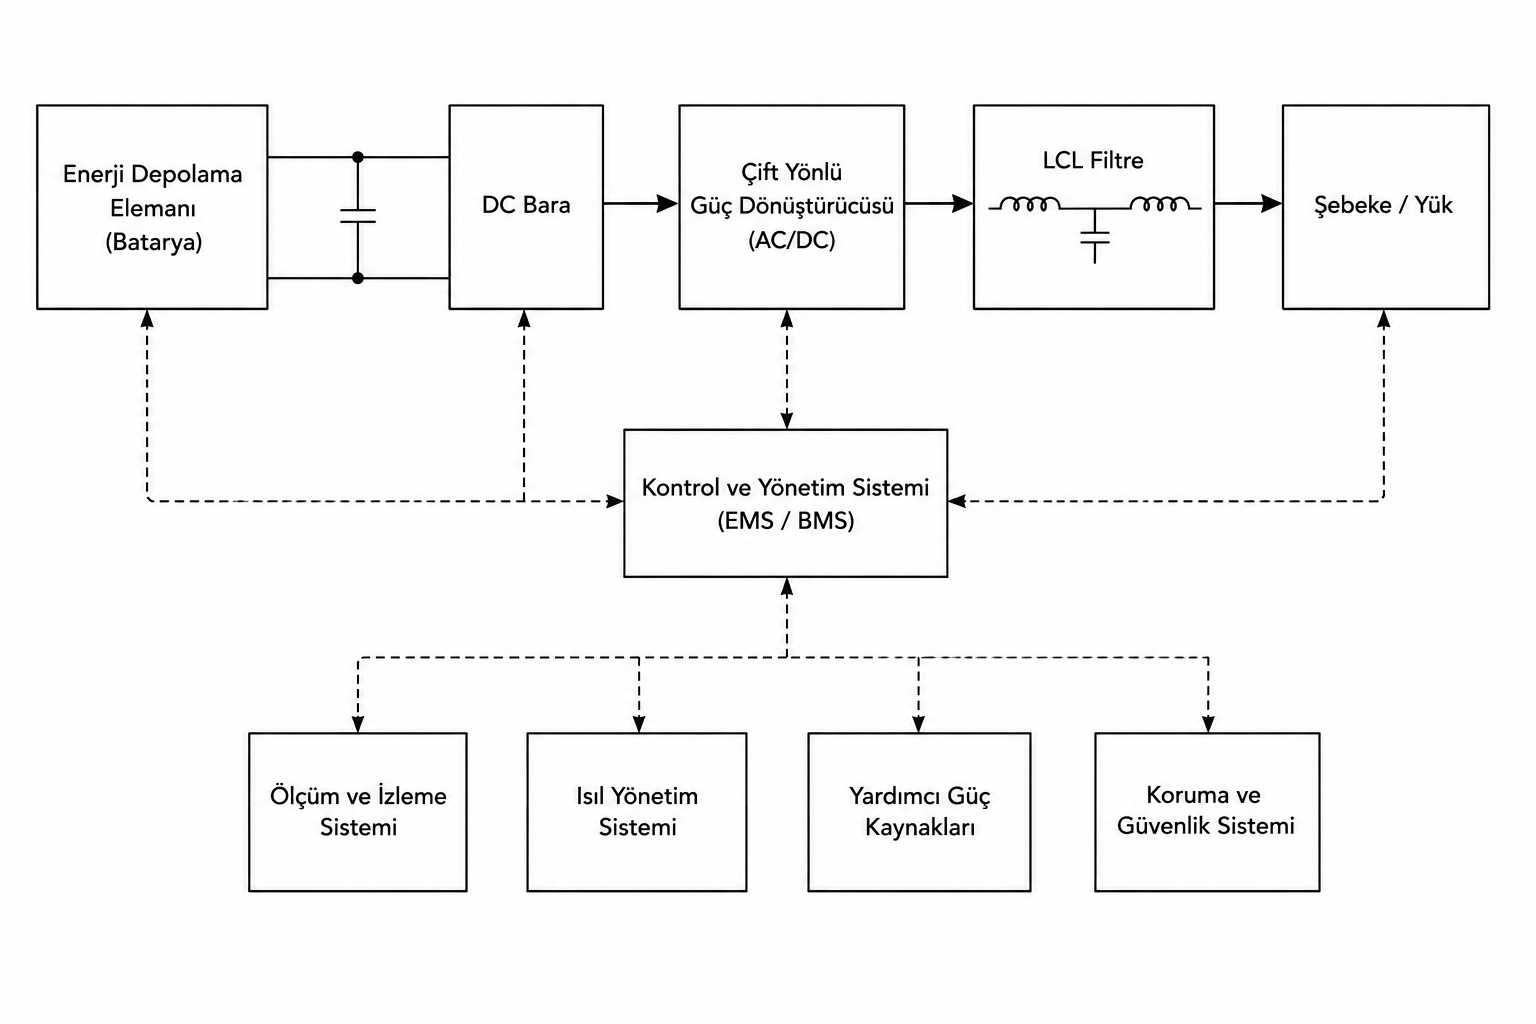
\includegraphics[width=0.96\textwidth]{literatur/gecici_eds_mimarisi_eski_tez.png}
  \caption{\eskitezetiketi\ Şebeke bağlantılı bir enerji depolama sisteminin temel bileşenleri ve bilgi akışları.}
  \label{fig:eds-mimarisi}
\end{figure}

Geleneksel şebeke bağlantılı bir EDS'de batarya ile DA bara arasında çift yönlü DA/DA dönüştürücü, DA bara ile şebeke arasında evirici/doğrultucu ve hücreler arasında ayrı bir dengeleme devresi bulunabilir. Katların ayrılması, her işlev için bağımsız tasarım ve koruma olanağı sunar; buna karşılık yarı iletken, manyetik eleman, sürücü, algılayıcı ve soğutma gereksinimini artırır. Sistem maliyeti çalışmalarında batarya paketi baskın kalem olsa da güç elektroniği donanımının maliyet, kayıp ve hacim üzerindeki etkisi ihmal edilemez \citep{Ramasamy2023,Lazard2024}. İşlevlerin ortak elemanlarla gerçekleştirilmesi, özellikle şarj ve deşarj kiplerinin aynı anda etkin olmadığı uygulamalarda donanım kullanım oranını yükseltme potansiyeli taşır.

\begin{table}[htbp]
  \centering
  \caption{\eskitezetiketi\ \diskaynaketiketi\ Enerji depolama sistemi bileşenlerinin toplam sistem maliyetindeki tipik pay aralıkları \citep{Ramasamy2023,Lazard2024}.}
  \label{tab:eds-maliyet-dagilimi}
  \begin{tabular}{>{\raggedright\arraybackslash}p{0.67\textwidth} c}
    \toprule
    \textbf{Sistem bileşeni} & \textbf{Maliyet payı (\%)} \\
    \midrule
    Batarya paketi & 50--70 \\
    Güç dönüştürücüleri (evirici, PFC ve DA/DA) & 10--20 \\
    Batarya yönetim sistemi & 3--8 \\
    Enerji yönetim sistemi & 2--5 \\
    Isıl yönetim ve soğutma & 3--10 \\
    Koruma ve güvenlik sistemleri & 2--5 \\
    Yardımcı güç kaynakları ve haberleşme & 1--3 \\
    Mekanik yapı ve kablolama & 5--10 \\
    \bottomrule
  \end{tabular}
\end{table}

Aralıkların toplamı tek bir tasarımı temsil etmediği için yüzde sütunu doğrudan toplanmamalıdır. Her satır farklı proje, güç ve tedarik koşullarından türetilen tipik bir aralıktır. Tablo~\ref{tab:eds-maliyet-dagilimi}, tezin GT-tipi mimarisindeki eleman paylaşımının neden ekonomik olarak anlamlı bir araştırma sorusu olduğunu gösterir; tek başına maliyet azalımını kanıtlamaz.

Batarya paketinin kullanılabilir ömrü; deşarj derinliği, hücre gerilimi, sıcaklık, akım oranı ve hücreler arası dengesizlikten etkilenir \citep{Vetter2005,Smith2017,Chen2021,Feng2018}. Önceki tezde kullanılan deşarj derinliği--çevrim ömrü eğrisi ile güvenli çalışma bölgesi Şekil~\ref{fig:batarya-omur-guvenlik} üzerinde korunmuştur. Eğriler belirli bir hücre kimyasının veri sayfası yerine literatürden uyarlanmış temsilî ilişkileri gösterdiğinden tasarım sınırı olarak kullanılmamalıdır.

\begin{figure}[htbp]
  \centering
  \begin{subfigure}[t]{0.49\textwidth}
    \centering
    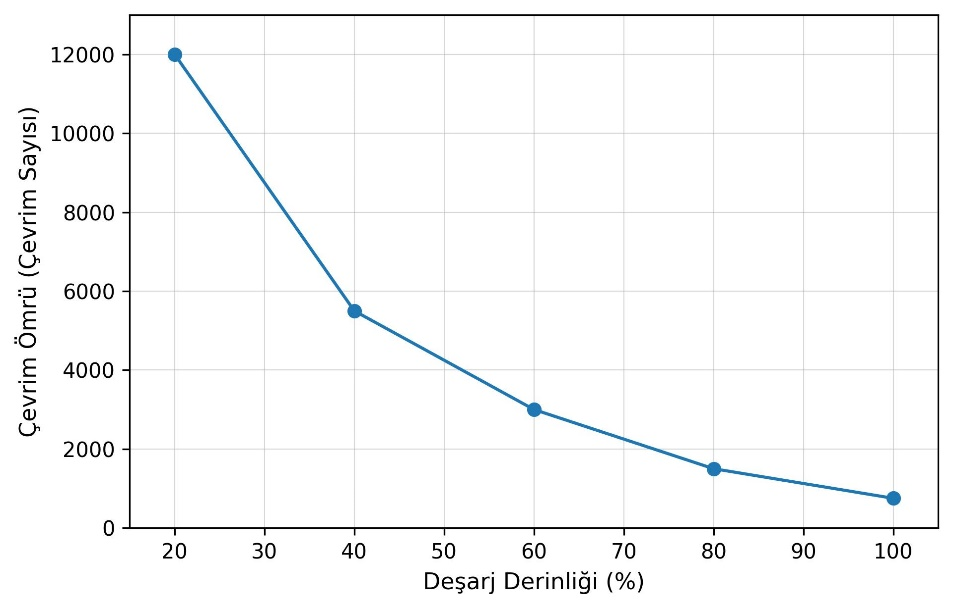
\includegraphics[width=\textwidth]{literatur/onceki_tez_dod_cevrim.jpg}
    \caption{Deşarj derinliği--çevrim ömrü ilişkisi.}
  \end{subfigure}\hfill
  \begin{subfigure}[t]{0.49\textwidth}
    \centering
    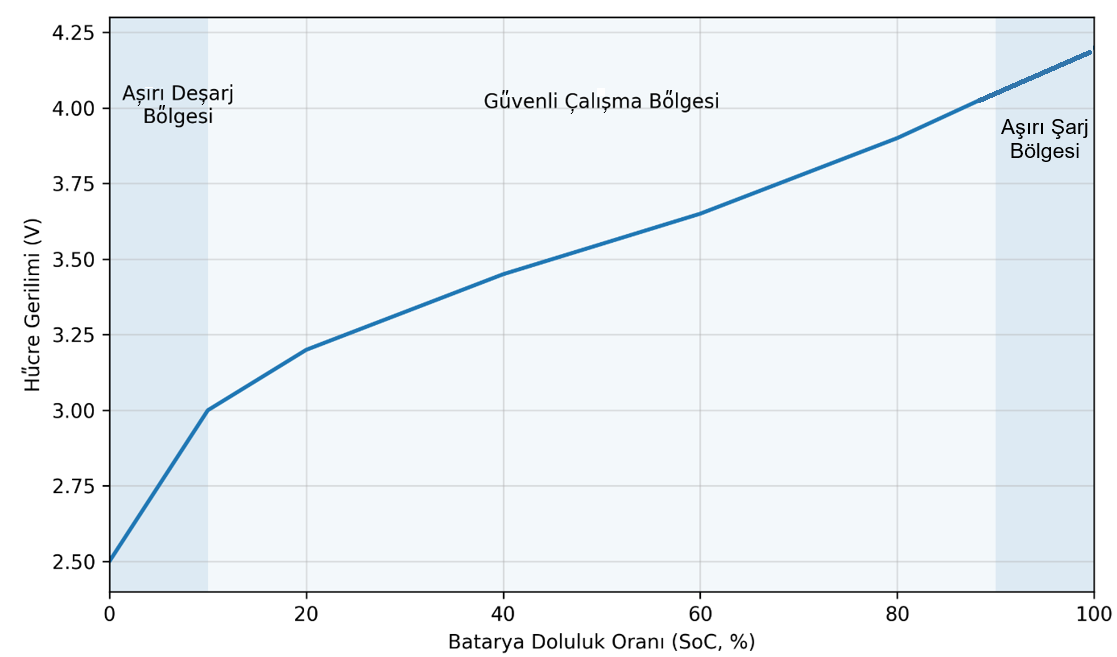
\includegraphics[width=\textwidth]{literatur/onceki_tez_guvenli_calisma.png}
    \caption{Temsilî gerilim ve doluluk sınırları.}
  \end{subfigure}
  \caption{\eskitezetiketi\ \diskaynaketiketi\ Batarya ömrü ve güvenli işletim için önceki tezde kullanılan temsilî eğriler; \citet{Smith2017}, \citet{Chen2021} ve \citet{Feng2018} temel alınarak uyarlanmıştır.}
  \label{fig:batarya-omur-guvenlik}
\end{figure}

Hücre gerilimi, akım ve sıcaklık ölçümleri BYS denetleyicisine taşınır; koruma, kontaktör ve dengeleme komutları aynı karar katmanında üretilir. Önceki tezdeki işlevsel BYS mimarisi Şekil~\ref{fig:bys-mimarisi} ile yeni bölüm yapısına aktarılmıştır. Mimari, GT-tipi yapının hangi işlevleri ortak güç elemanlarına taşımayı hedeflediğini tanımlayan başvuru noktasıdır.

\begin{figure}[htbp]
  \centering
  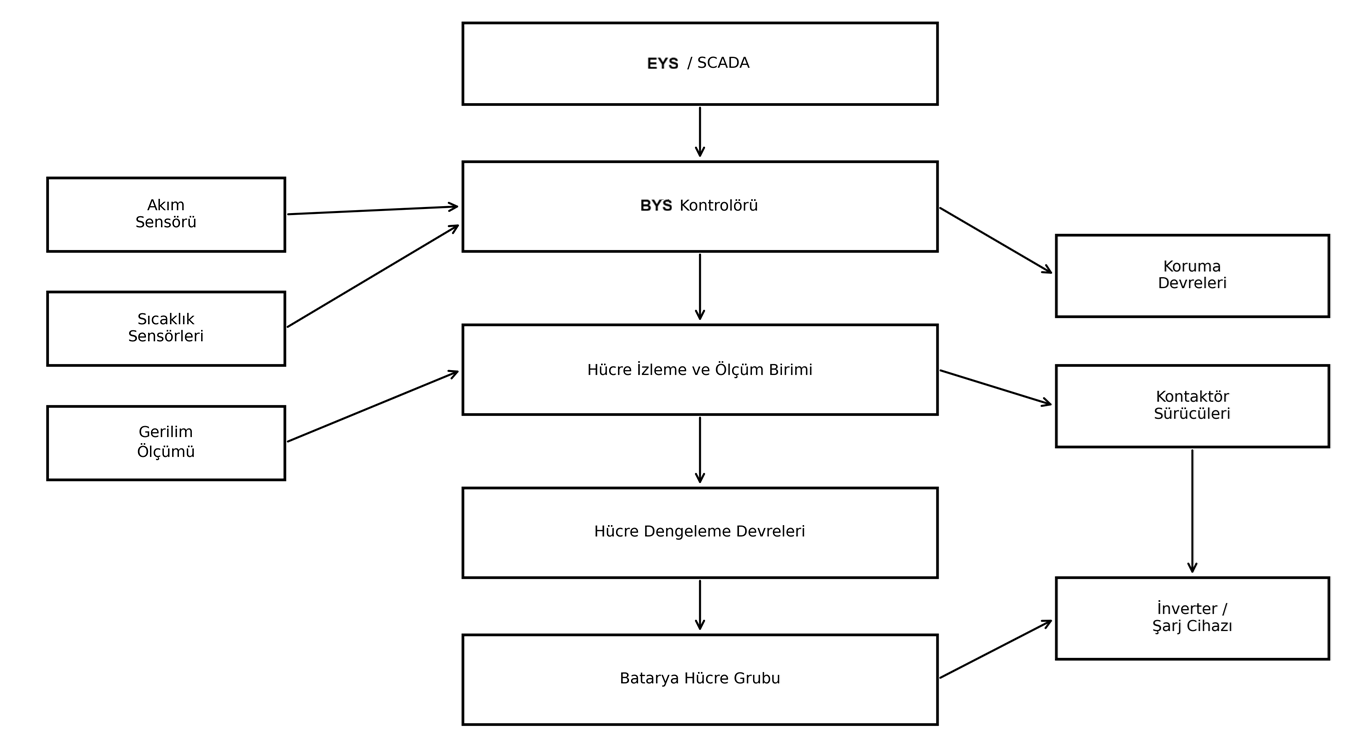
\includegraphics[width=0.94\textwidth]{literatur/onceki_tez_bys_mimarisi.png}
  \caption{\eskitezetiketi\ Tipik bir batarya yönetim sisteminin ölçüm, karar, koruma ve dengeleme işlevleri.}
  \label{fig:bys-mimarisi}
\end{figure}

\begin{table}[htbp]
  \centering
  \caption{\eskitezetiketi\ Geleneksel BYS ile hücre bazlı enerji yönetiminin işlevsel karşılaştırması.}
  \label{tab:bys-islev-karsilastirma}
  \setlength{\tabcolsep}{4pt}
  \begin{tabularx}{\textwidth}{>{\raggedright\arraybackslash}X >{\centering\arraybackslash}p{0.22\textwidth} >{\centering\arraybackslash}p{0.25\textwidth}}
    \toprule
    \textbf{İşlev} & \textbf{Geleneksel BYS} & \textbf{Hücre bazlı yönetim} \\
    \midrule
    Hücre izleme, koruma ve dengeleme & Var & Var \\
    Hücre bazlı şarj kontrolü & Sınırlı & Var \\
    Hücre bazlı deşarj kontrolü & Sınırlı & Var \\
    Ömür optimizasyonu & Dolaylı & Doğrudan \\
    \bottomrule
  \end{tabularx}
\end{table}

Tablo~\ref{tab:bys-islev-karsilastirma}'daki ``doğrudan'' ifadesi bir ömür kazancı yüzdesi değil, hücrenin güç yoluna ayrı ayrı müdahale edilebilmesini tanımlar. Sayısal ömür artışı ancak hücre kimyası, görev profili, sıcaklık ve yaşlanma testi birlikte verildiğinde ileri sürülebilir.

Seri bağlı hücre veya modüllerde kapasite, iç direnç, sıcaklık ve yaşlanma farklılıkları paket performansını en zayıf birimle sınırlandırabilir. Pasif dengeleme fazla enerjiyi dirençlerde harcarken aktif dengeleme kapasitör, endüktör, transformatör veya çift yönlü dönüştürücü üzerinden enerji aktarır \citep{Daowd2011,Khan2024}. Aktif yöntemler enerji kaybını azaltabilse de ilave anahtar ve manyetik eleman gereksinimi doğurur. Literatürdeki yeniden yapılandırılabilir batarya sistemleri, hücre veya modül bağlantılarını güç anahtarlarıyla değiştirerek dengeleme, arıza yalıtımı ve farklı terminal gerilimlerini aynı donanım üzerinden sağlamayı hedeflemektedir. Momayyezan ve arkadaşları, yüksek gerilimli batarya sisteminde yük besleme, geri kazanım, şarj ve modüller arası dengeleme kipleri için yarı iletkenleri ve bir endüktörü paylaşan bütünleşik bir dönüştürücü önermiş ve beş modüllü ölçekli prototiple çalışma kiplerini göstermiştir \citep{Momayyezan2016}. Farakhor ve arkadaşları ise yeniden yapılandırılabilir anahtar dizisini hücre düzeyindeki DA/DA dönüştürücülerle birleştirerek arızalı hücre yalıtımı, güç paylaşımı, şarj durumu ve sıcaklık dengelemesi sağlamış; yaklaşımı benzetim ve laboratuvar prototipiyle doğrulamıştır \citep{Farakhor2023}.

Pasif ve başlıca aktif dengeleme ailelerinin enerji aktarım elemanları Şekil~\ref{fig:dengeleme-yontemleri} üzerinde karşılaştırılmıştır. Şekil, yöntemlerin ayrıntılı devre tasarımından çok enerji yolundaki temel farkı göstermek amacıyla verilmiştir.

\begin{figure}[htbp]
  \centering
  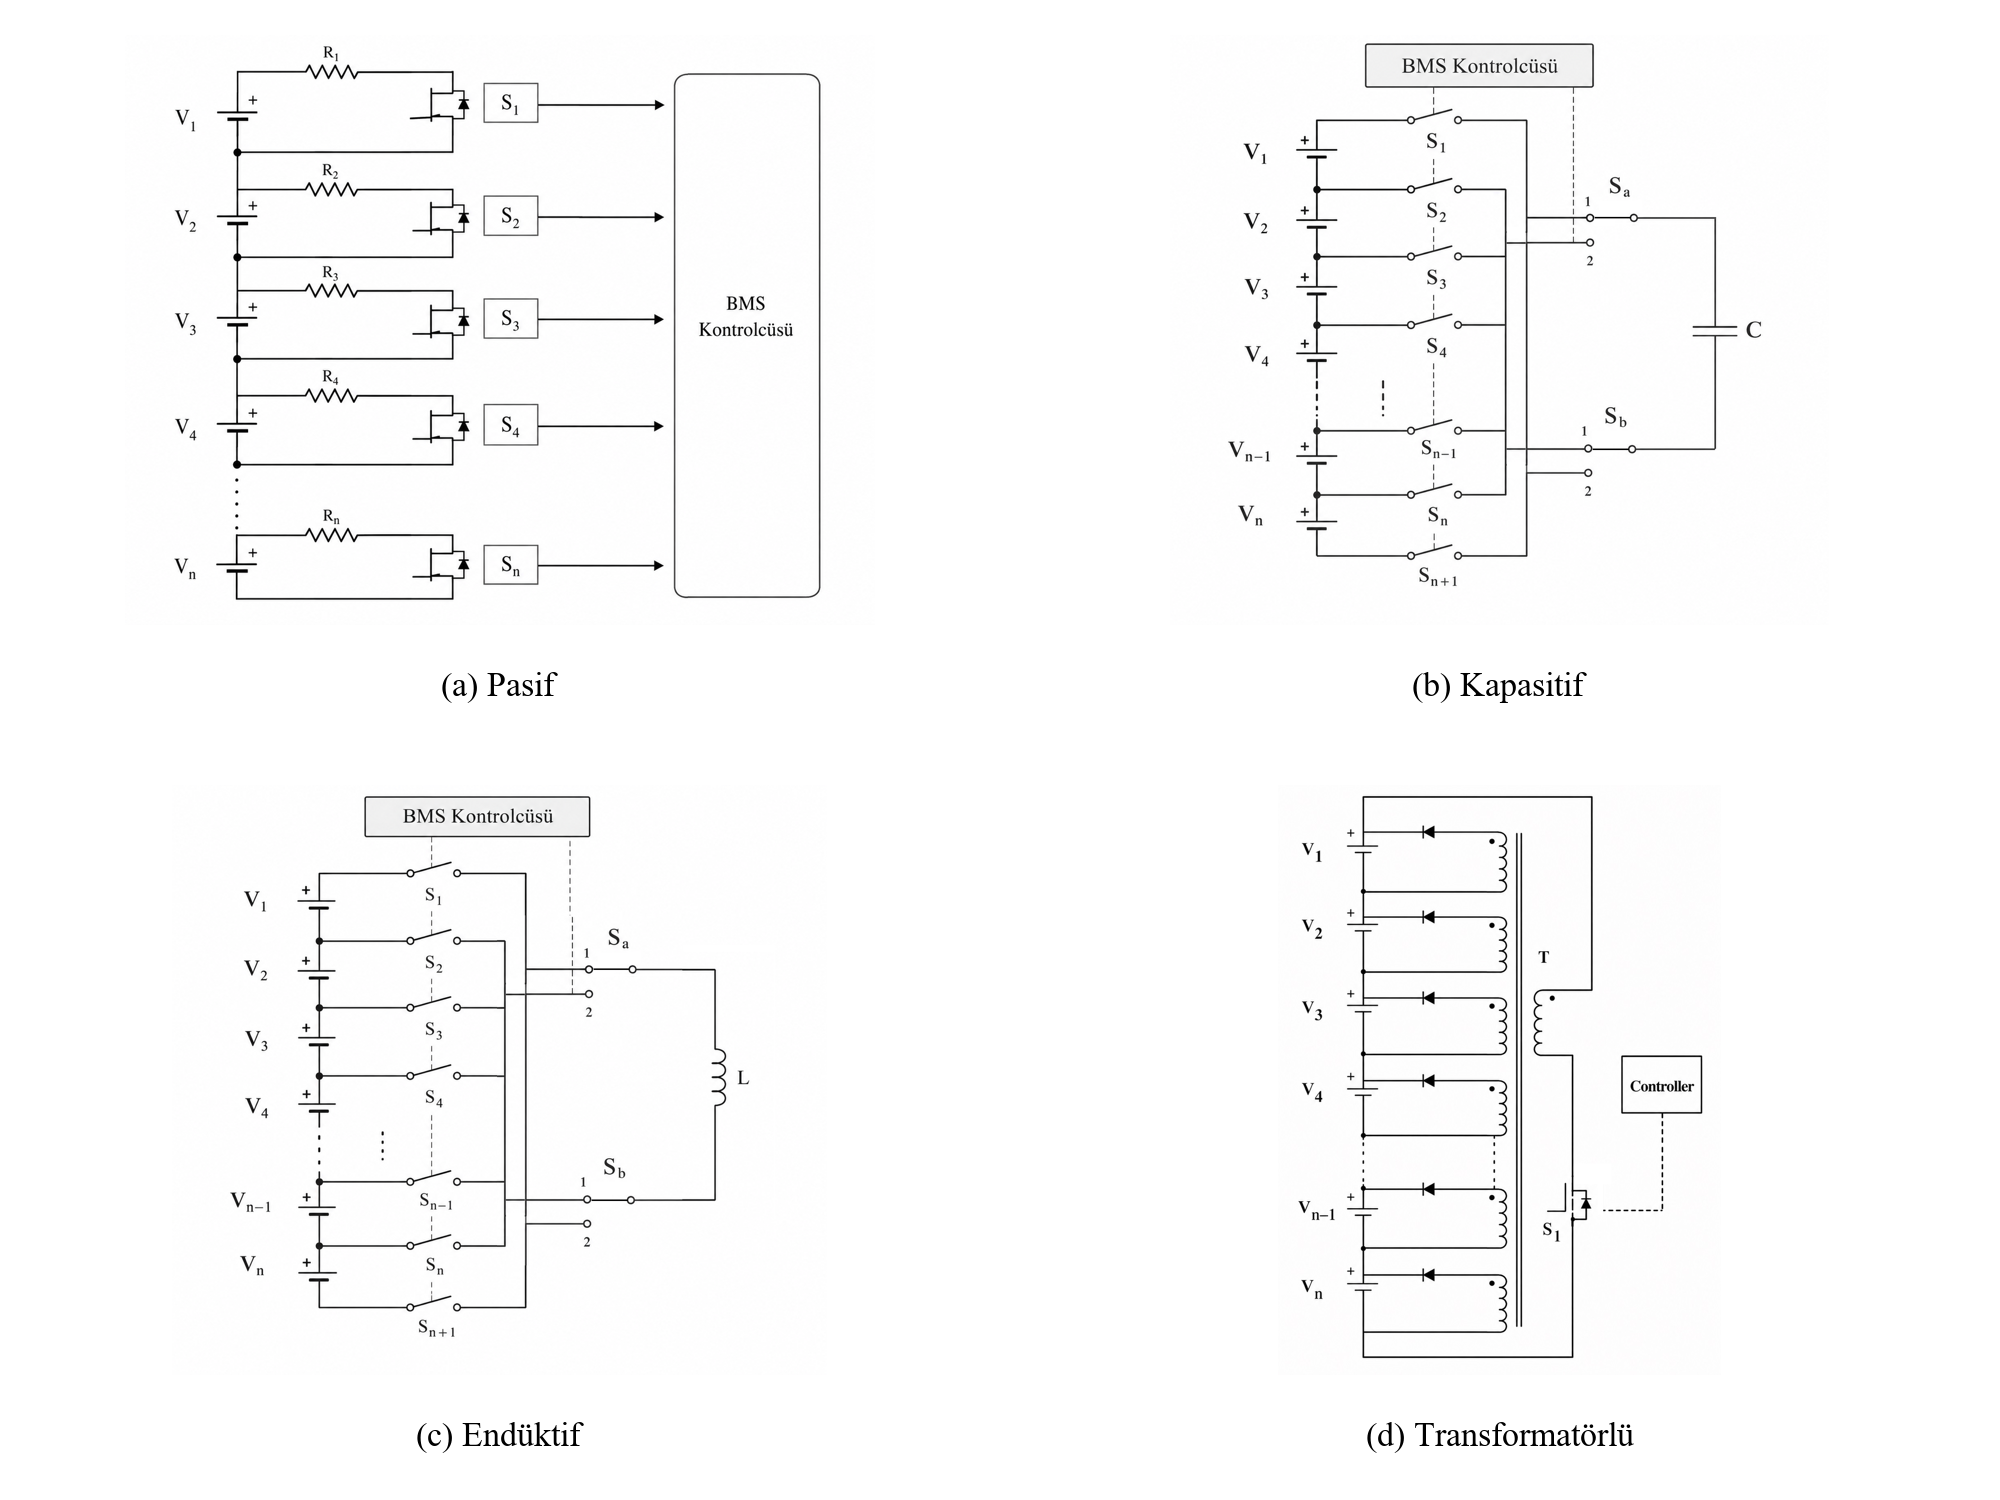
\includegraphics[width=0.94\textwidth]{literatur/gecici_dengeleme_yontemleri_bilesik.png}
  \caption{\eskitezetiketi\ Pasif, kapasitif, endüktif ve transformatörlü hücre dengeleme yapılarının kavramsal karşılaştırması \citep{Daowd2011,Khan2024}.}
  \label{fig:dengeleme-yontemleri}
\end{figure}

Pasif dengeleme yönteminde, diğer hücrelere göre daha yüksek gerilim veya şarj durumuna sahip hücreye paralel bağlanan direnç üzerinden enerji harcanır. Anahtarın görev oranı hücreden çekilen dengeleme akımını belirler. Az sayıda eleman, basit denetim ve düşük maliyet başlıca avantajlardır. Fazla enerjinin ısıya dönüştürülmesi, soğutma gereksinimi ve düşük şarj durumundaki hücrelere enerji aktarılamaması ise yöntemin temel sınırlılıklarını oluşturur \citep{Daowd2011,Khan2024}.

Kapasitif dengelemede, anahtarlanan bir kapasitör farklı hücrelere sırasıyla bağlanarak gerilimi yüksek hücreden enerji alır ve gerilimi düşük hücreye aktarır. Manyetik eleman gerektirmeyen yapı, paketleme ve maliyet bakımından avantaj sağlayabilir. Dengeleme akımının hücreler arasındaki gerilim farkına bağlı olması, uzak hücreler arasında enerjinin birden fazla aktarım adımından geçmesi ve anahtar sayısının hücre sayısıyla artması dengeleme süresini uzatabilir \citep{Daowd2011,Khan2024}.

Endüktif dengeleme yönteminde enerji, anahtarlama sırasında bir endüktörde depolanır ve seçilen hücreye veya paket hattına kontrollü akım olarak aktarılır. Anahtarlama görev oranı üzerinden enerji akışının düzenlenebilmesi, kapasitif yönteme göre daha yüksek ve öngörülebilir dengeleme akımlarına olanak tanır. Endüktör, akım algılama, sürücü ve çift yönlü anahtarlama gereksinimleri devre ile denetim karmaşıklığını artırır \citep{Daowd2011,Khan2024}.

Transformatörlü yapılarda hücre sargıları ile ortak sargı arasındaki manyetik bağ, hücreden pakete, paketten hücreye veya seçilen hücreler arasında yalıtımlı enerji aktarımı sağlayabilir. Çoklu sargı yapısı farklı enerji yollarını desteklediği için hücre bazlı şarj ve deşarj işlevlerine geçiş bakımından önemlidir. Sargı sayısı, kaçak endüktans, sürme düzeni, hacim ve üretim maliyeti uygulama büyüdükçe belirleyici sınırlılıklara dönüşür \citep{Daowd2011,Khan2024}.

\begin{table}[htbp]
  \centering
  \caption{\eskitezetiketi\ \diskaynaketiketi\ Başlıca hücre dengeleme ailelerinin nitel karşılaştırması \citep{Daowd2011,Khan2024}.}
  \label{tab:dengeleme-karsilastirma}
  \setlength{\tabcolsep}{3pt}
  \begin{tabularx}{\textwidth}{>{\raggedright\arraybackslash}p{0.20\textwidth} *{4}{>{\centering\arraybackslash}X}}
    \toprule
    \textbf{Yöntem} & \textbf{Enerji geri kazanımı} & \textbf{Maliyet} & \textbf{Karmaşıklık} & \textbf{Aktarım hızı} \\
    \midrule
    Pasif & Yok & Düşük & Düşük & Düşük \\
    Anahtarlamalı kapasitör & Var & Düşük--orta & Orta & Düşük--orta \\
    Endüktif & Var & Orta & Yüksek & Orta--yüksek \\
    Transformatörlü & Var & Yüksek & Yüksek & Uygulamaya bağlı \\
    \bottomrule
  \end{tabularx}
\end{table}

Nitel sınıflar topoloji, hücre sayısı ve dengeleme akımıyla değişebildiğinden Tablo~\ref{tab:dengeleme-karsilastirma} kesin bir sıralama değil, tasarım alanını özetleyen bir karşılaştırmadır. Önceki tezdeki ``verim'' ve ``güç seviyesi'' gibi bağlamsız nitelemeler, doğrudan ölçülebilir ``enerji geri kazanımı'' ve ``aktarım hızı'' başlıklarıyla yeniden ifade edilmiştir.

Dört yöntem birlikte değerlendirildiğinde tek bir dengeleme yapısının verim, hız, maliyet ve devre karmaşıklığı açısından her uygulamada üstün olmadığı görülür. Tezin GT-tipi mimari katkısı, söz konusu yöntemlerden birini genel olarak en iyi ilan etmek yerine, şarj--deşarj ve hücre yönetimi işlevlerinde mevcut yarı iletkenlerin yeniden görevlendirilmesine odaklanmaktadır. Dolayısıyla Şekil~\ref{fig:dengeleme-yontemleri}, ilerleyen bölümlerde sunulan işlev paylaşımının neden ayrı dengeleme donanımına alternatif oluşturabileceğini açıklayan kuramsal geçiş niteliğindedir.

Yeniden yapılandırılabilir sistemlerin esneklik kazancı yeni tasarım ödünleşimleri oluşturur. Anahtar sayısı yükseldikçe iletim kaybı, sürücü karmaşıklığı, yanlış anahtarlama riski ve güvenli kip geçişi gereksinimi büyür. Huang ve arkadaşlarının modüler yeniden yapılandırılabilir EDS çalışması, üç anahtarlı modül yapısıyla farklı bağlantıları ve arıza yalıtımını desteklerken işlev sayısı ile devre karmaşıklığı arasındaki ödünleşimi açıkça göstermiştir \citep{Huang2024}. Sonuç olarak bütünleştirme, yalnızca eleman sayısını azaltma iddiasıyla değerlendirilemez; her çalışma kipi için akım yolu, eleman zorlanması, geçiş sırası, kayıp ve doğrulama düzeyi birlikte verilmelidir.

\tezcalismanotu{D2-1 --- Eski EDS/BYS içeriğinin birleştirme denetimi}{Eski Şekil~1.2--1.3 tek batarya ömrü/güvenlik görselinde, eski Şekil~1.6--1.9 ise tek dengeleme karşılaştırmasında birleştirilmiştir. Nihai teslimde özgün dört dengeleme devresinden bağlantı, anahtar yönü veya enerji aktarım yolu bakımından kaybolan ayırt edici ayrıntı bulunup bulunmadığı tekrar denetlenecek; gerekirse ayrıntılı devreler Ek~A'ya taşınacaktır. Eski Şekil~1.10'daki göreli ömür senaryosu, yaşlanma denklemi ve kaynak veri bulunmadığı için alınmamıştır; model bulunursa MATLAB'da yeniden üretilecek, bulunmazsa çıkarma gerekçesi korunacaktır.}

\section{Üç Seviyeli T-Tipi Dönüştürücünün Kuramsal Temeli}

Gerilim kaynaklı iki seviyeli evirici, faz çıkışını DA baranın pozitif ve negatif uçları arasında anahtarlar. Yüksek anahtarlama frekansı akım dalgalanmasını ve filtre gereksinimini azaltırken anahtarlama kayıplarını artırır. Çok seviyeli dönüştürücüler, çıkış gerilimini daha küçük basamaklarla oluşturarak yarı iletken gerilim zorlanmasını, $dv/dt$ değerini ve filtreleme gereksinimini azaltmayı amaçlar \citep{Mohan2003,Holmes2003}. Üç seviyeli nötr nokta kenetlemeli (NPC) yapı, sıfır seviyesini kenetleme diyotlarıyla üretirken T-tipi yapı nötr noktayı çift yönlü kontrollü bir anahtar kolu üzerinden faz çıkışına bağlar.

Bir T-tipi faz kolunda dış anahtarlar faz düğümünü DA baranın pozitif veya negatif yarısına, nötr anahtar çifti ise orta noktaya bağlar. İdeal anahtarlama durumları $+V_{\mathrm{dc}}/2$, $0$ ve $-V_{\mathrm{dc}}/2$ seviyelerini oluşturur. Pozitif ve negatif aktif durumlarda akım dış anahtarlar üzerinden, sıfır durumunda ise akım yönüne bağlı olarak nötr kol üzerinden akar. Nötr kol elemanlarının daha düşük gerilim sınıfında seçilebilmesi ile aktif durumdaki seri eleman sayısının NPC yapıya göre azalması, uygun gerilim ve anahtarlama frekansı aralığında iletim ve anahtarlama kayıpları açısından avantaj sağlayabilir.

T-tipi faz kolunun temel devre yapısı Şekil~\ref{fig:t-tipi-faz-kolu} üzerinde gösterilmiştir. Sonraki bölümlerde aynı devre, her anahtarlama durumu için akım yönleri işaretlenerek ayrıntılandırılacaktır.

\begin{figure}[htbp]
  \centering
  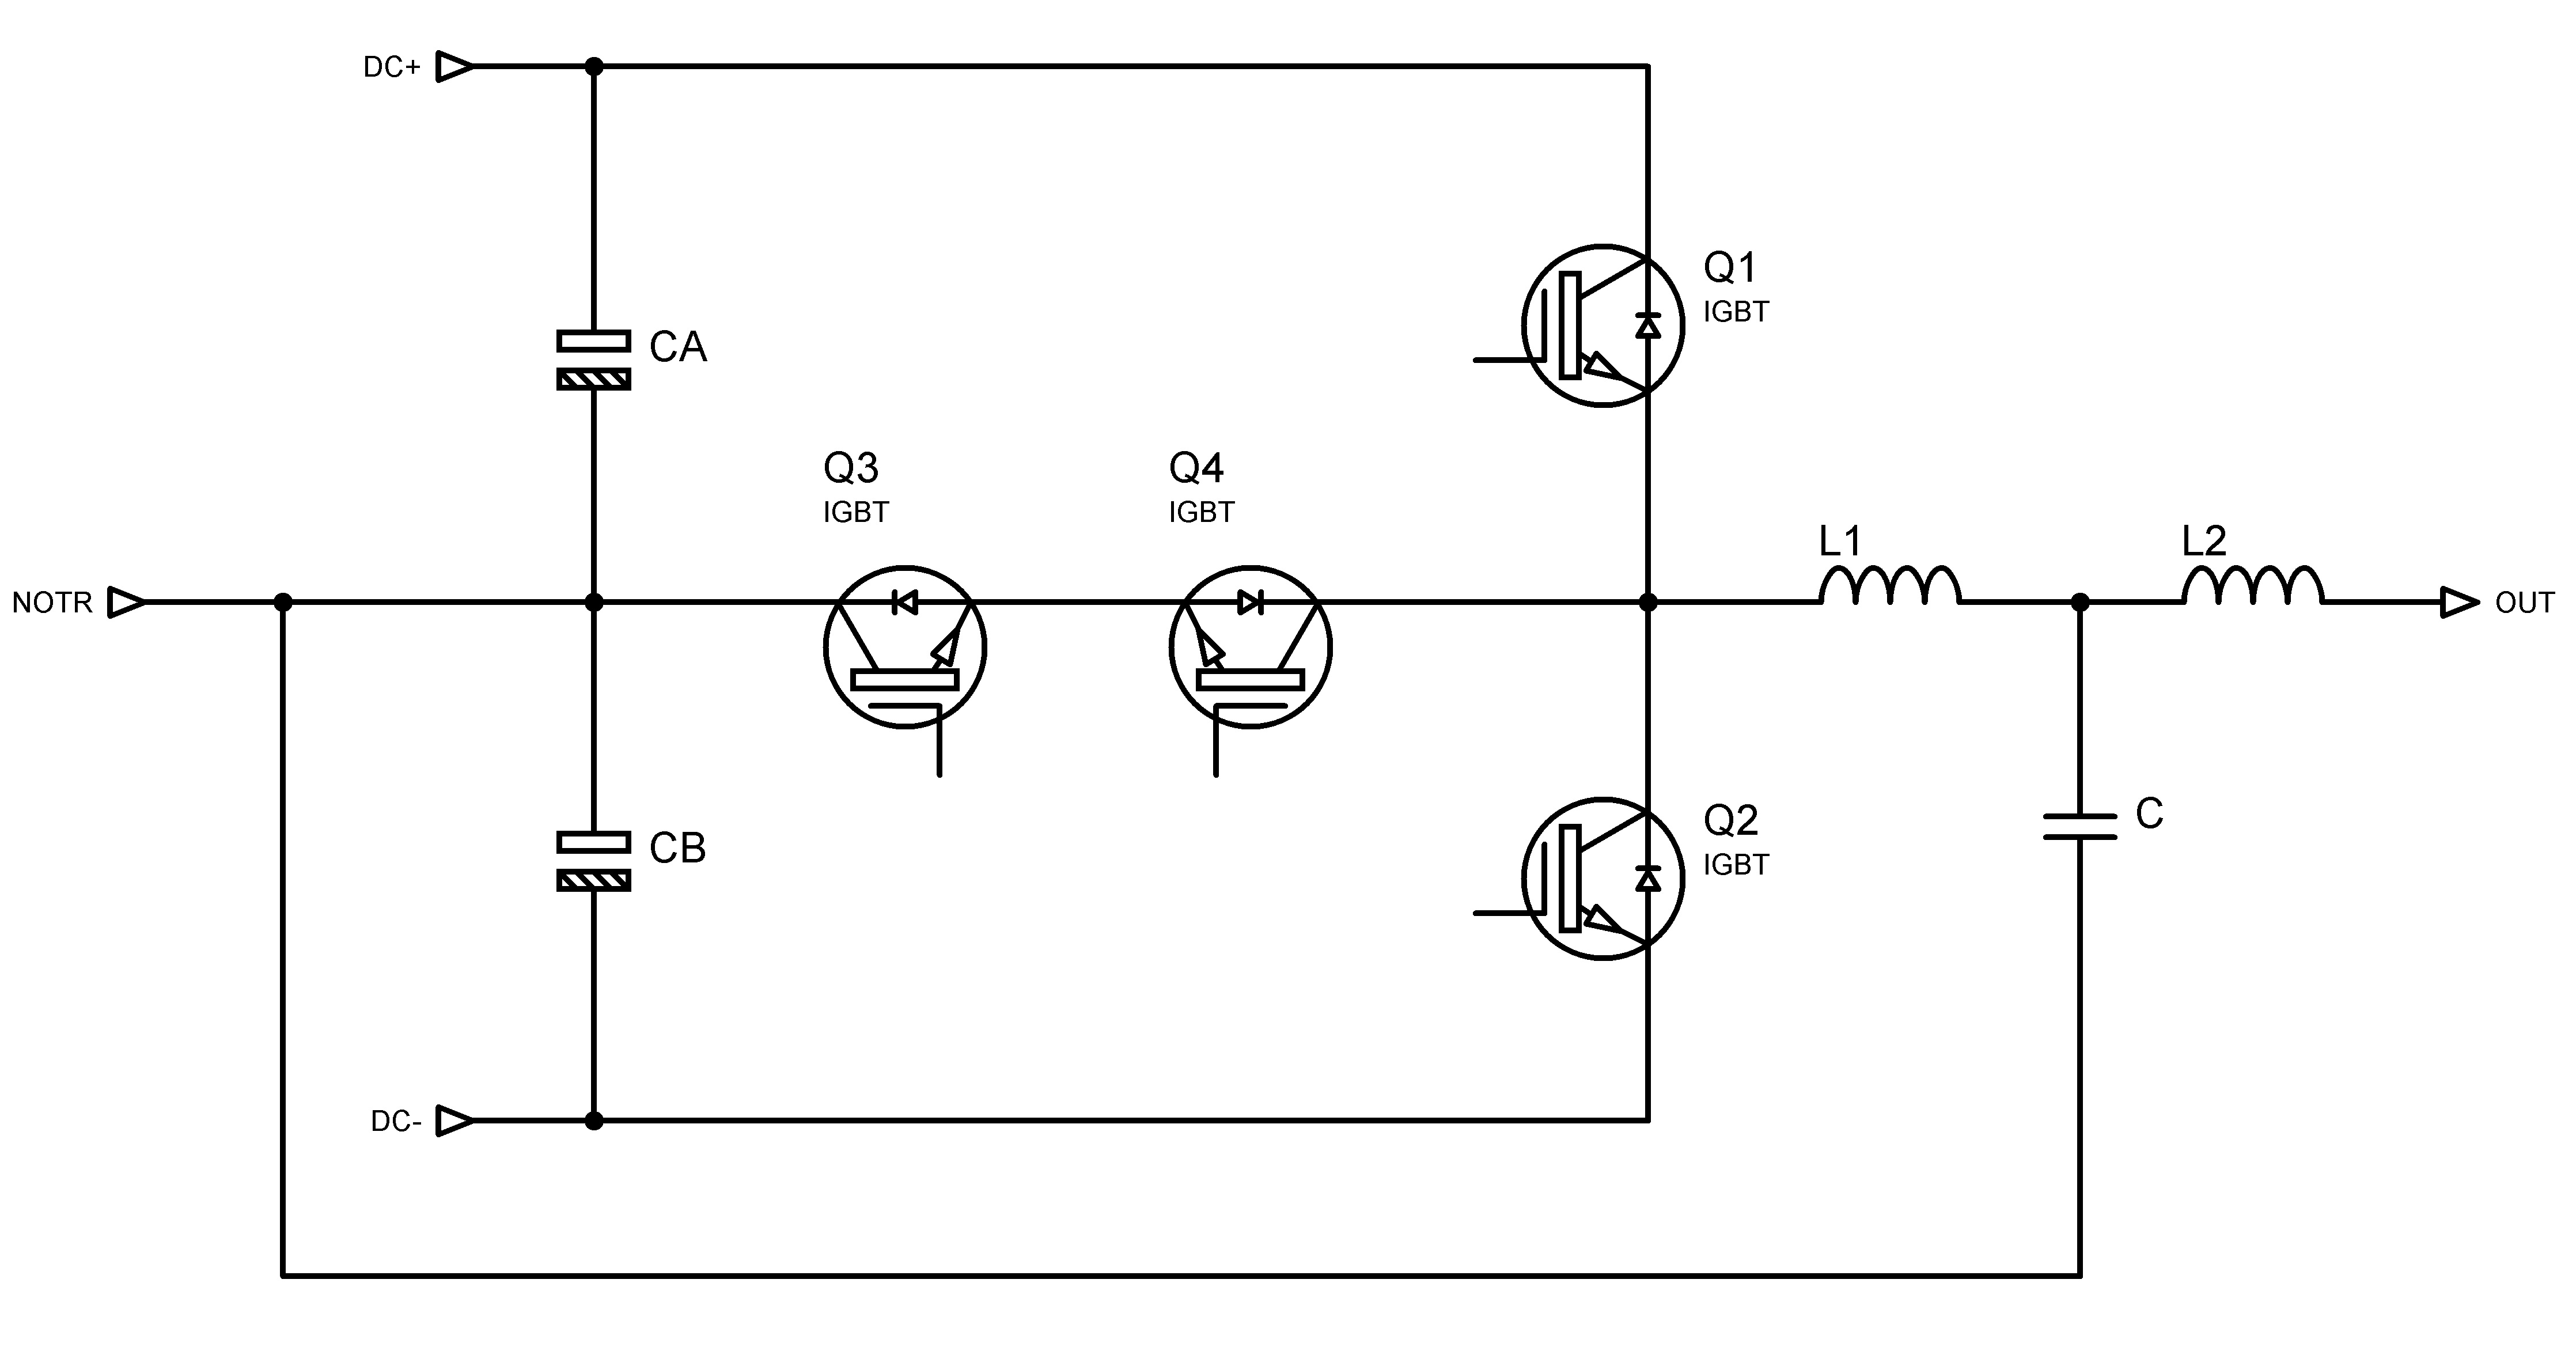
\includegraphics[width=0.88\textwidth]{literatur/gecici_t_tipi_faz_kolu_eski_tez.jpg}
  \caption{\eskitezetiketi\ Üç seviyeli T-tipi eviricinin tek faz kolu ve çıkış filtresi.}
  \label{fig:t-tipi-faz-kolu}
\end{figure}

Schweizer ve Kolar, üç seviyeli T-tipi dönüştürücüyü iki seviyeli ve NPC seçenekleriyle yarı iletken kaybı, eleman alanı ve deneysel verim bakımından karşılaştırmış; düşük gerilim uygulamalarında yüksek anahtarlama frekansına rağmen yüksek verim elde edilebildiğini göstermiştir \citep{Schweizer2013}. Wang ve arkadaşlarının \SI{250}{\kilo\watt} SiC T-tipi evirici çalışması, çalışma aralıklarını ve anahtarlama geçişlerini ayrıntılı biçimde çözümleyerek ters iletimin eleman kayıpları üzerindeki etkisini modellemiş; \SI{25}{\kilo\watt\per\litre} güç yoğunluğu hedefli bir prototip sunmuştur \citep{Wang2020}. Hizarci ve arkadaşlarının \SI{25}{\kilo\watt}, \SI{15}{\kilo\hertz} şebeke bağlantılı T-tipi evirici üzerindeki iletilen emisyon çalışması ise topolojinin endüstriyel ölçekte filtre, kaçak akım ve elektromanyetik uyumluluk gereksinimleriyle birlikte ele alınması gerektiğini göstermektedir \citep{Hizarci2021}.

T-tipi topolojiye ilişkin çalışmaların önemli bölümü anma gücü, yüksek güç yoğunluğu, yarı iletken seçimi, nötr nokta dengesi ve modülasyon üzerine yoğunlaşmaktadır. Harmonik eleme amaçlı anahtarlama açıları ve üçüncü harmonik enjeksiyonu da DA bara kullanımını veya belirli gerilim harmoniklerini iyileştirmek amacıyla incelenmiştir \citep{Aghdam2013,Holmes2003}. Söz konusu çalışmalar topolojinin genel verim ve dalga biçimi potansiyelini ortaya koymakla birlikte, şebekeye bağlı düşük akım koşulunda nötr kolun ters akım oluşturma mekanizmasını ve verim--THD ödünleşimini doğrudan merkezine almamaktadır.

\section{Fotovoltaik Çalışma Profili, Kısmi Yükte Verim ve Harmonik Bozulma}

Fotovoltaik üretimin ışınım ve sıcaklığa bağlı değişimi, şebeke eviricisinin geniş bir güç aralığında çalışmasına neden olur. Önceki tezdeki günlük profil, aylık ışınım dizisi ve bunlardan türetilen 144 çalışma noktası Şekil~\ref{fig:fv-calisma-profilleri} üzerinde MATLAB ile yeniden üretilmiştir. PVGIS, konum, yönelim, eğim, sistem kaybı ve meteorolojik veri kümesi belirtilerek saatlik veya aylık üretim hesabı yapılmasına olanak tanır \citep{Taylor2025PVGIS}. Eski dosyada söz konusu sorgunun konumu ve ham çıktısı bulunmadığından ilk iki grafik ölçülmüş saha verisi değil, temsilî profil olarak adlandırılmıştır.

\begin{figure}[htbp]
  \centering
  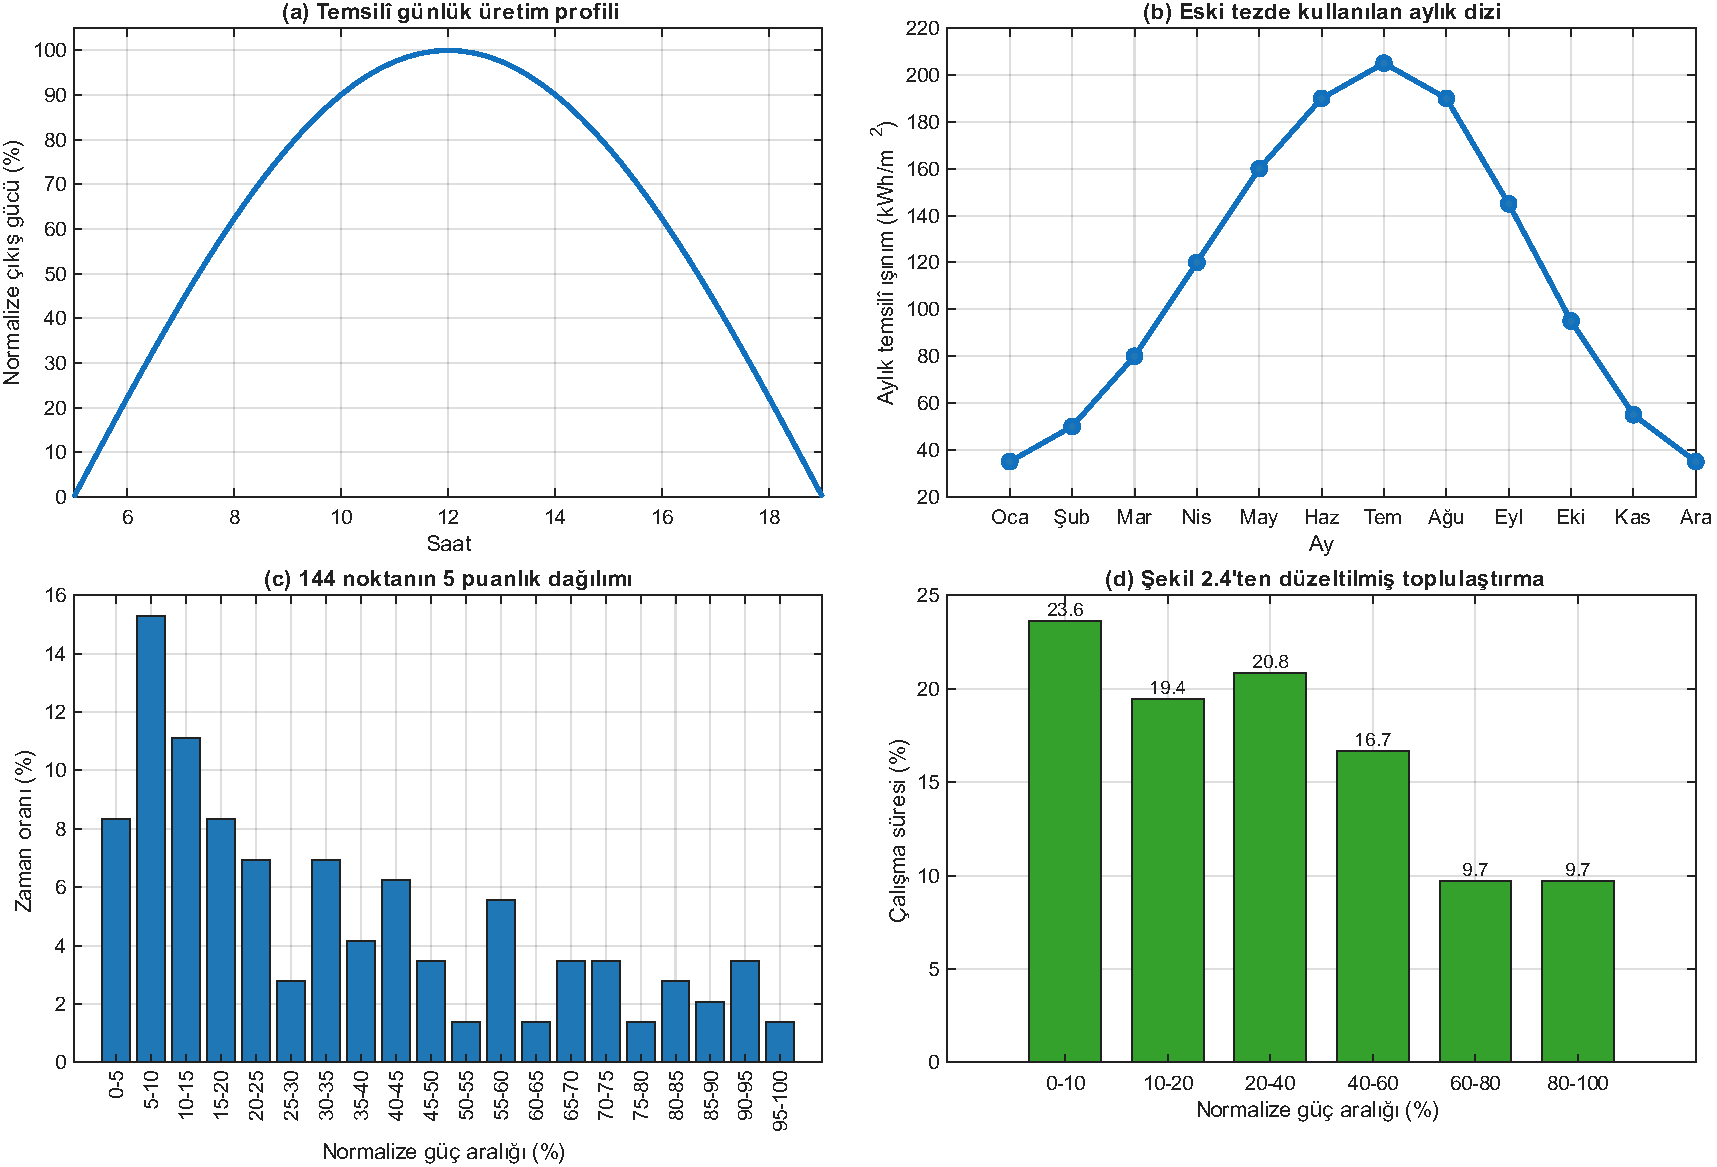
\includegraphics[width=\textwidth]{literatur/matlab_b2_guc_profilleri.pdf}
  \caption{\eskitezetiketi\ \juriistegietiketi\ Önceki tezdeki temsilî günlük ve aylık FV profilleri ile 144 çalışma noktasının MATLAB'da yeniden üretilen güç dağılımı. (d) paneli, eski Tablo~2.1'deki tutarsız yüzdeler yerine (c) panelindeki nokta sayılarının yeniden gruplanmasıyla elde edilmiştir.}
  \label{fig:fv-calisma-profilleri}
\end{figure}

\juriistegietiketi\ \small Jürinin genelden özele akış, akademik kanıt ve okunur şekil talepleri doğrultusunda eski raster grafikler beyaz zeminli vektör PDF olarak yeniden üretilmiş; hesap ile kaynak verisi arasındaki ayrım açıkça belirtilmiştir.

\normalsize
Önceki tezde Şekil~2.1 ve Şekil~2.2 olarak verilen günlük ve aylık diziler arasındaki çarpım bağı, eski Şekil~2.3'ün doğrudan aktarımıyla Şekil~\ref{fig:fv-yil-saat-yuzeyi} üzerinde korunmuştur. Saat indisi $h$, ay indisi $m$, boyutsuz gün içi normalize profil $p_d(h)$ ve aya bağlı temsilî ışınım seviyesi $G_m(m)$ ile gösterilsin. Aynı birimi $G_m$'den alan temsilî yıl--saat ışınımı $G_{\mathrm{tem}}(m,h)$
\begin{equation}
G_{\mathrm{tem}}(m,h)=G_m(m)\,p_d(h)
\label{eq:temsili-yil-saat-yuzeyi}
\end{equation}
biçiminde tanımlanır. Eşitlik~\eqref{eq:temsili-yil-saat-yuzeyi} ölçülmüş bir saha modeli değil, iki normalize dizinin çarpımıdır. Fotovoltaik gücün ışınımla orantılı olduğu basitleştirilmiş kabul altında $P_{\mathrm{tem}}(m,h)/P_n\approx G_{\mathrm{tem}}(m,h)/G_{\max}$ bağıntısı elde edilir; burada $P_{\mathrm{tem}}$ temsilî gücü, $P_n$ anma gücünü ve $G_{\max}$ yüzeydeki en büyük ışınımı gösterir. Önceki tez grafiğindeki yaklaşık \SI{4}{\watt\per\metre\squared} ve \SI{200}{\watt\per\metre\squared} uçları, temsilî örneklemde 50 katlık bir çalışma aralığına ve en düşük sıfırdan farklı noktanın tepe değerin yaklaşık \SI{2}{\percent}'sine karşılık geldiğine işaret etmektedir.

\begin{figure}[htbp]
  \centering
  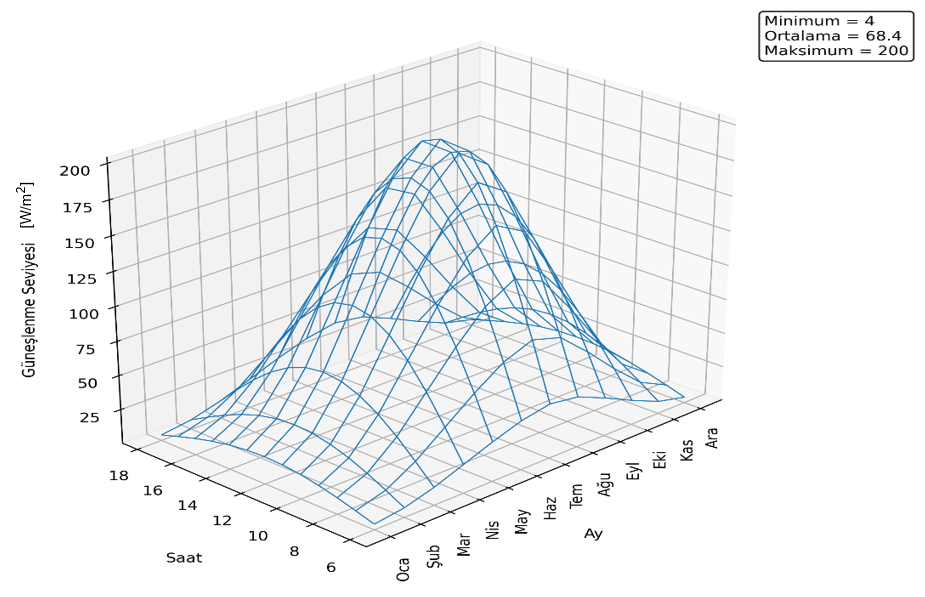
\includegraphics[width=0.86\textwidth]{literatur/onceki_tez_yil_saat_uretim_yuzeyi.png}
  \caption{\eskitezetiketi\ Önceki tezde günlük ve aylık temsilî dizilerin çarpımından elde edilen yıl--saat ışınım/üretim yüzeyi. Konum ve ham PVGIS sorgusu bulunmadığından yüzey ölçülmüş yıllık üretim değil, düşük güç çalışma aralığını göstermek için kullanılan temsilî bir türetimdir.}
  \label{fig:fv-yil-saat-yuzeyi}
\end{figure}

Şekil~\ref{fig:fv-yil-saat-yuzeyi}, günlük ve aylık profillerden güç sınıfı dağılımına geçişi görünür kıldığı için bölümde tutulmuştur. Konum, panel eğimi, sıcaklık, sistem kayıpları, ardışık hava koşulları ve gerçek zaman ağırlıkları hesaba katılmadığından yüzey yıllık enerji hesabı ya da saha ölçümü olarak yorumlanmamalıdır. Dolayısıyla yüzeyin kullanımı, önceki tezdeki örnekleme mantığını ve düşük güç çalışma aralığını gösteren temsilî bir türetimle sınırlandırılmıştır.

Şekil~\ref{fig:fv-calisma-profilleri}(c)'deki sayımlar 144 temsilî çalışma noktasına karşılık gelmektedir. İlk iki güç sınıfında toplam 34 nokta bulunması, eşit ağırlıklı ay--saat örneklemi içindeki noktaların \SI{23.6}{\percent}'sının anma gücünün \SI{10}{\percent}'undan düşük olduğunu gösterir. Söz konusu oran gerçek yıllık çalışma süresini değil, önceki tezde kullanılan temsilî örnekleme düzeninin dağılımını ifade etmektedir. Üç yıllık saha verisine dayanan bir çalışma, ışınımın önemli bir bölümünün düşük ve orta seviyelerde gerçekleştiğini; düşük ışınım ile evirici eşik kayıplarının sistem performansını etkilediğini göstermiştir \citep{Mondol2007}. Farklı iklim koşullarında yürütülen ağırlıklı verim incelemesi de yalnızca tepe veriminin saha davranışını temsil etmeye yetmediğini, evirici performansının değişen ışınım ve kısmi yük seviyeleriyle birlikte değerlendirilmesi gerektiğini ortaya koymuştur \citep{AbRahman2020}. Dolayısıyla \SI{23.6}{\percent} değeri evrensel bir yıllık oran olarak değil, düşük güç bölgesinin incelenmesini motive eden eski tez örnekleminin sonucu olarak kullanılmaktadır.

\begin{table}[htbp]
  \centering
  \caption{\eskitezetiketi\ \juriistegietiketi\ Eski Şekil~2.4'teki 144 noktanın düzeltilmiş güç sınıfı dağılımı.}
  \label{tab:fv-guc-dagilimi}
  \begin{tabular}{ccc}
    \toprule
    \textbf{Çıkış gücü ($\%P_n$)} & \textbf{Nokta sayısı} & \textbf{Temsilî oran (\%)} \\
    \midrule
    0--10 & 34 & 23,6 \\
    10--20 & 28 & 19,4 \\
    20--40 & 30 & 20,8 \\
    40--60 & 24 & 16,7 \\
    60--80 & 14 & 9,7 \\
    80--100 & 14 & 9,7 \\
    \midrule
    Toplam & 144 & 100,0 \\
    \bottomrule
  \end{tabular}
\end{table}

Yıllık enerji verimi yalnızca tepe verimle belirlenmediğinden Avrupa ve CEC ağırlıklı verim tanımları, farklı yük noktalarındaki dönüşüm verimlerini belirli katsayılarla birleştirir. Alt indis $x$, anma gücünün yüzde $x$ noktasını; $\eta_x$ ise aynı noktadaki dönüşüm verimini göstersin. Avrupa ağırlıklı verimi
\begin{equation}
\eta_{\mathrm{EU}}=0{,}03\eta_{5}+0{,}06\eta_{10}+0{,}13\eta_{20}+0{,}10\eta_{30}+0{,}48\eta_{50}+0{,}20\eta_{100}
\label{eq:eta-eu}
\end{equation}
ve CEC ağırlıklı verimi
\begin{equation}
\eta_{\mathrm{CEC}}=0{,}04\eta_{10}+0{,}05\eta_{20}+0{,}12\eta_{30}+0{,}21\eta_{50}+0{,}53\eta_{75}+0{,}05\eta_{100}
\label{eq:eta-cec}
\end{equation}
olarak tanımlanır \citep{Sera2008,Sandia2015}. Eşitlik~\eqref{eq:eta-eu} ve Eşitlik~\eqref{eq:eta-cec} içindeki katsayıların toplamı birdir; dolayısıyla iki ifade de boyutsuz ağırlıklı ortalamadır. Deneysel test düzenekleri ve standartlaştırılmış protokoller, verimin güç seviyesi, giriş gerilimi ve MPPT koşullarıyla birlikte ölçülmesini öngörür \citep{Sera2008,Sandia2015}. İzmir ışınım verilerine dayalı çalışma da bölgesel güç dağılımının ağırlık katsayılarını değiştirebildiğini göstermiştir \citep{Ongun2013}.

\begin{table}[htbp]
  \centering
  \caption{\eskitezetiketi\ \diskaynaketiketi\ Avrupa ve CEC ağırlıklı verim katsayıları \citep{Sera2008,Sandia2015}.}
  \label{tab:agirlikli-verim-katsayilari}
  \begin{tabular}{c*{6}{c}}
    \toprule
    \textbf{Yöntem} & \multicolumn{6}{c}{\textbf{Güç seviyesi ve ağırlık katsayısı}} \\
    \midrule
    Avrupa & $5:0{,}03$ & $10:0{,}06$ & $20:0{,}13$ & $30:0{,}10$ & $50:0{,}48$ & $100:0{,}20$ \\
    CEC & $10:0{,}04$ & $20:0{,}05$ & $30:0{,}12$ & $50:0{,}21$ & $75:0{,}53$ & $100:0{,}05$ \\
    \bottomrule
  \end{tabular}
\end{table}

Eski tezdeki tipik verim--güç ve THD--güç dizileri ile bu dizilerin 144 noktaya uygulanmasından elde edilen sınıf oranları Şekil~\ref{fig:fv-verim-thd-profilleri} üzerinde korunmuştur. Paneller (a) ve (c) genel eğilimi gösteren önceki tez dizileridir; belirli bir ürünün doğrulanmış veri sayfası veya yeni deney sonucu değildir. Paneller (b) ve (d) aynı dizilerden türetilen ikincil hesaplardır ve tez katkısının performans kanıtı olarak kullanılmayacaktır.

\begin{figure}[H]
  \centering
  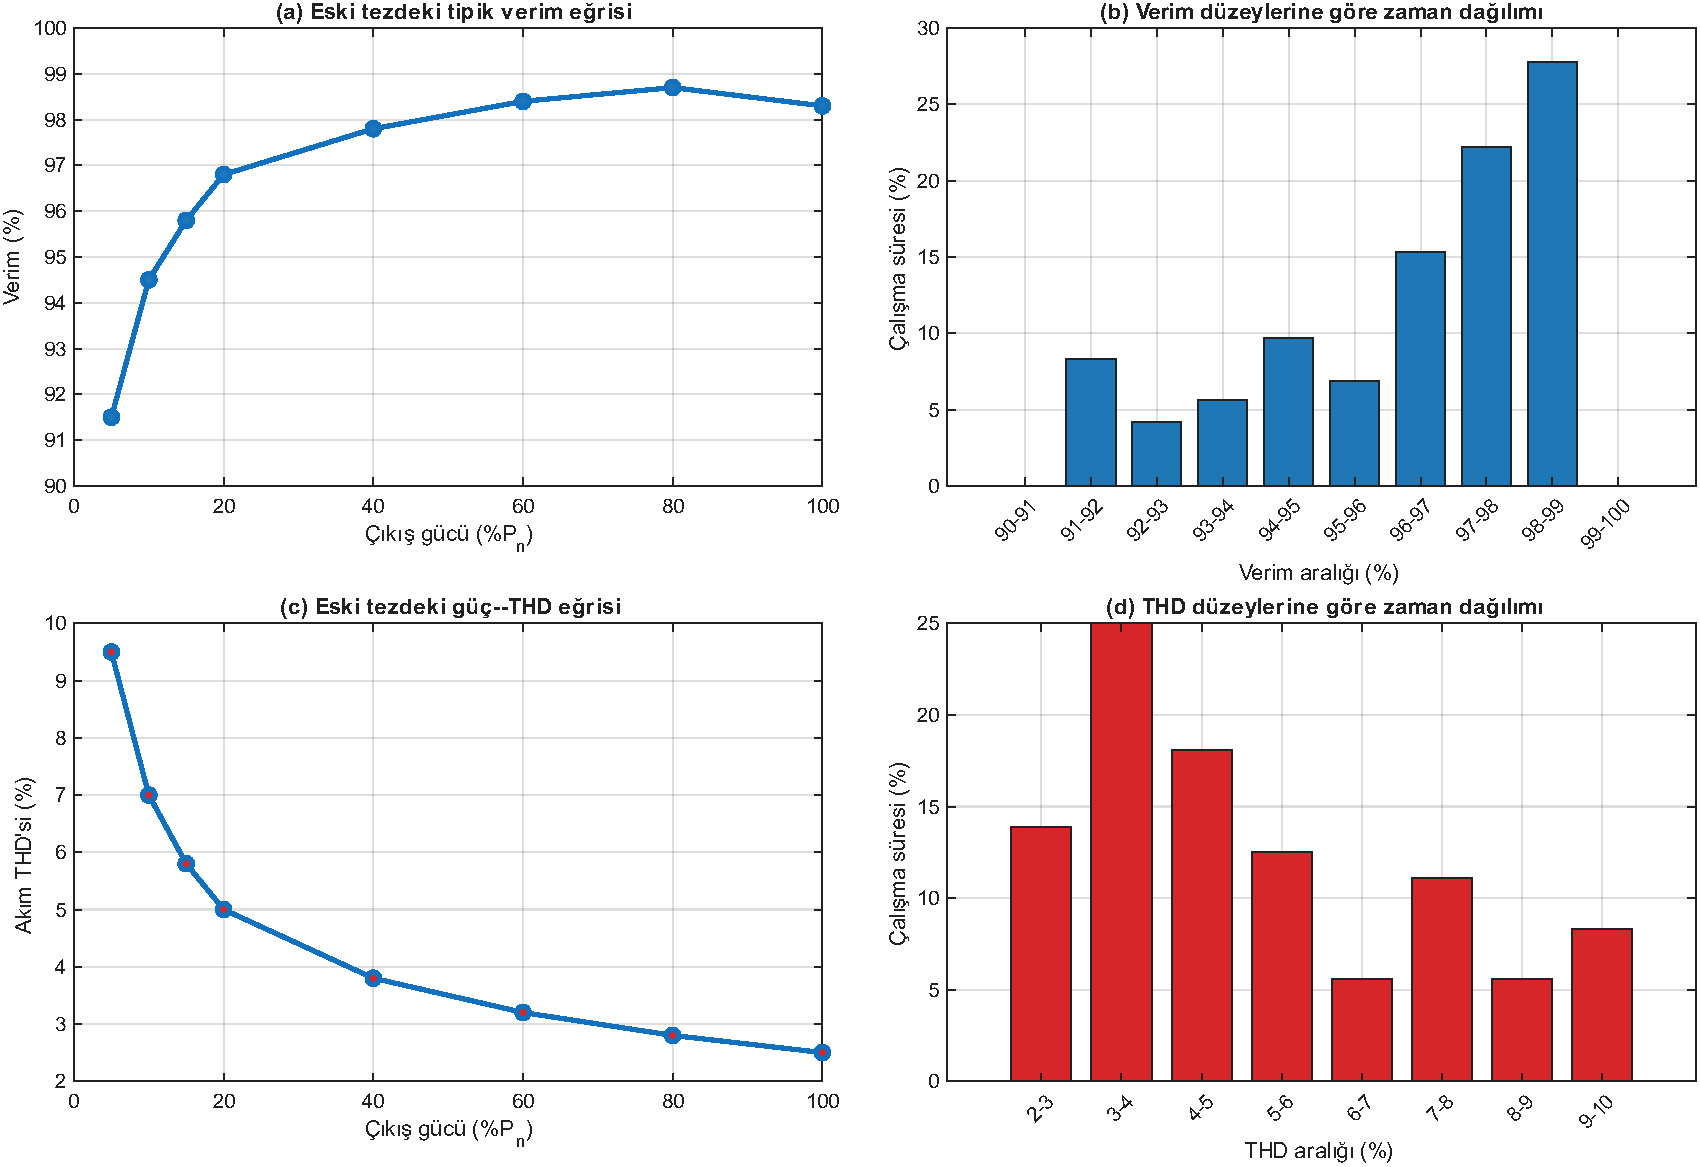
\includegraphics[width=\textwidth]{literatur/matlab_b2_verim_thd_profilleri.pdf}
  \caption{\eskitezetiketi\ \juriistegietiketi\ Önceki tezdeki tipik kısmi yük verim ve THD eğrileri ile bunlardan türetilen temsilî zaman dağılımlarının MATLAB'da vektörel yeniden üretimi.}
  \label{fig:fv-verim-thd-profilleri}
\end{figure}

Şekil~\ref{fig:fv-verim-thd-profilleri}(a)'daki önceki tez dizisinde verim, \SI{5}{\percent} yükte yaklaşık \SI{91.5}{\percent}, \SI{10}{\percent} yükte \SI{94.5}{\percent} ve \SI{80}{\percent} yükte \SI{98.7}{\percent} düzeyindedir. Aynı şeklin (c) panelinde akım THD'si \SI{5}{\percent} yükte \SI{9.5}{\percent}, \SI{20}{\percent} yükte \SI{5.0}{\percent} ve anma gücünde \SI{2.5}{\percent} olarak verilmiştir. Paneller (b) ve (d), söz konusu eğrileri 144 temsilî çalışma noktasına uygulayarak düşük güç bölgesinin toplu sonuç üzerindeki ağırlığını göstermektedir. Şeklin bölümdeki amacı, yalnızca tepe veriminin ve anma gücündeki THD'nin yıllık davranışı açıklamaya yetmediğini ortaya koymaktır; sayısal diziler kaynak cihaz ve ham ölçüm bulunmadan yeni tasarımın doğrulanması olarak kullanılmayacaktır.

Düşük güçte THD artışının dış literatür kanıtı, \citet{Chicco2009} tarafından raporlanan günlük güç ve akım THD kaydıyla Şekil~\ref{fig:chicco-guc-thd} üzerinde gösterilmiştir. Sabah ve akşam düşük güç bölgelerinde THD'nin yükselmesi, tezin kısmi yük odağını destekler; belirli harmoniklerin T-tipi nötr kol mekanizmasından kaynaklandığını tek başına kanıtlamaz.

\begin{figure}[H]
  \centering
  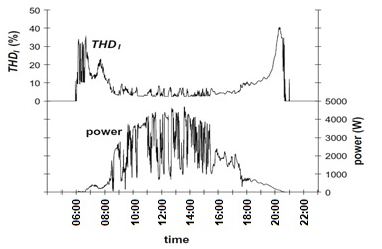
\includegraphics[width=0.62\textwidth]{literatur/chicco2009_guc_thd.png}
  \caption{\diskaynaketiketi\ \SI{5}{\kilo\watt} sınıfındaki bir FV eviricinin gün içi çıkış gücü ve akım THD'si; \citet{Chicco2009}'dan alınmıştır.}
  \label{fig:chicco-guc-thd}
\end{figure}

Önceki tezde ayrıca şebekeye bağlı \SI{10}{\kilo\watt} sınıfındaki ticari bir eviricinin sabah devreye giriş kaydı verilmiştir. Tablo~\ref{tab:ticari-evirici-thd} sayısal kaydı korumaktadır. Cihaz seri numarası, güç analizörü, örnekleme penceresi, şebeke gerilimi ve ham dosya bulunmadığından satırlar yeni deney kanıtı değil, doğrulanmayı bekleyen önceki tez kaydıdır.

\begin{table}[H]
  \centering
  \caption{\eskitezetiketi\ Ticari eviricinin sabah devreye girişinde kaydedildiği belirtilen güç ve akım THD değerleri; ham ölçüm dosyası ve protokolü doğrulanacaktır.}
  \label{tab:ticari-evirici-thd}
  \begin{tabular}{lrrr}
    \toprule
    \textbf{Zaman} & \textbf{Güç (W)} & \textbf{Güç ($\%P_n$)} & \textbf{THD (\%)} \\
    \midrule
    Devreye ilk giriş & 100 & 1,00 & 400 \\
    07:50 & 500 & 5,00 & 34 \\
    08:00 & 580 & 5,80 & 27 \\
    08:10 & 729 & 7,29 & 26 \\
    08:35 & 1060 & 10,60 & 17 \\
    08:50 & 1320 & 13,20 & 14 \\
    09:05 & 1450 & 14,50 & 14 \\
    09:18 & 1720 & 17,20 & 13 \\
    09:26 & 1880 & 18,80 & 9 \\
    09:42 & 2200 & 22,00 & 8 \\
    \bottomrule
  \end{tabular}
\end{table}

\begin{figure}[H]
  \centering
  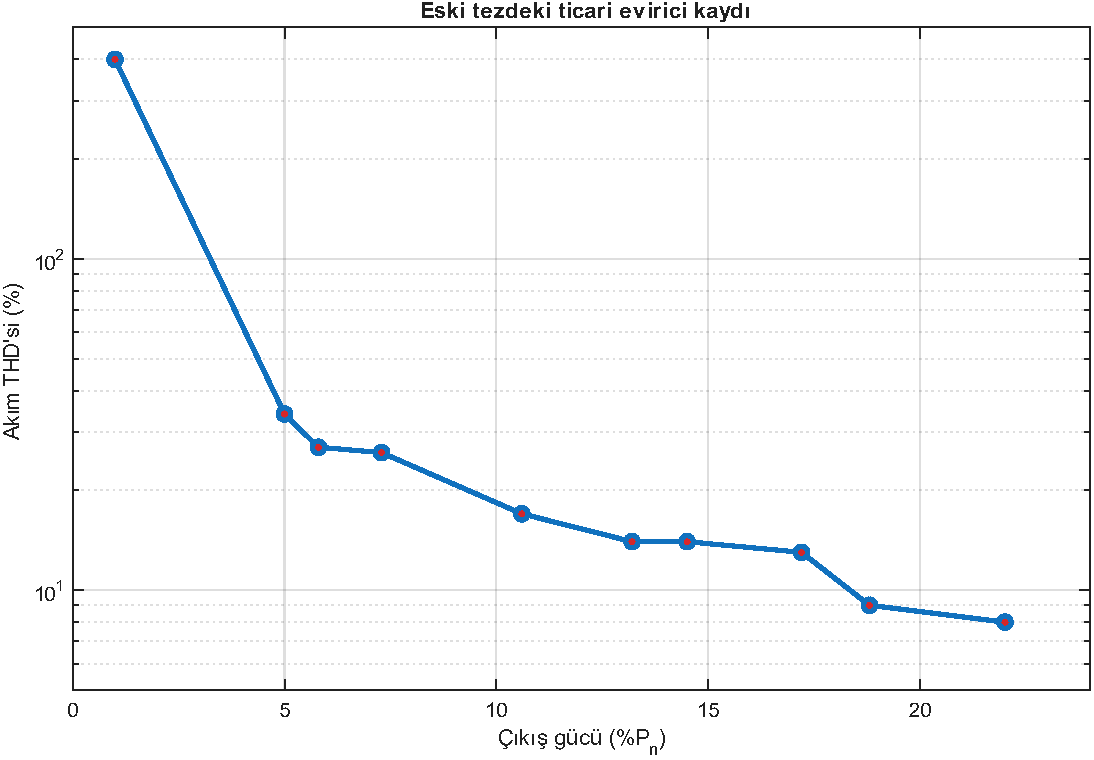
\includegraphics[width=0.84\textwidth]{literatur/matlab_b2_ticari_evirici_thd.pdf}
  \caption{\eskitezetiketi\ \juriistegietiketi\ Tablo~\ref{tab:ticari-evirici-thd}'deki önceki tez kaydının MATLAB'da yeniden çizimi; düşey eksen logaritmiktir ve veri doğrulanmayı beklemektedir.}
  \label{fig:ticari-evirici-thd}
\end{figure}

Şekil~\ref{fig:ticari-evirici-thd}, önceki tez kaydındaki doğrusal olmayan azalmayı logaritmik eksende görünür hâle getirmektedir. Kayıtta akım THD'si anma gücünün \SI{1}{\percent}'inde \SI{400}{\percent}, \SI{5}{\percent}'inde \SI{34}{\percent}, \SI{18.8}{\percent}'inde \SI{9}{\percent} ve \SI{22}{\percent}'inde \SI{8}{\percent} olarak verilmiştir. Grafiğin bölümde tutulma nedeni, devreye giriş ve düşük güç test noktalarının yalnızca anma gücündeki tek bir ölçümle temsil edilemeyeceğini göstermektir. Doğrulanmamış ticari evirici kaydı önerilen anahtarlama yönteminin başarısını kanıtlamaz; yeni deneylerde karşılaştırma noktalarının seçimini gerekçelendiren tarihsel gözlem niteliğindedir.

Düşük güçte sürücü, kontrol, anahtarlama ve manyetik elemanların güce zayıf bağlı kayıpları toplam çıkışa oranla büyür. Şebeke akımının küçük olması, ölü zaman ve anahtar doğrusal olmayanlıklarının temel bileşene oranını da artırır. Saha ve laboratuvar ölçümleri, FV eviricilerde akım dalga biçimi bozulmasının güç seviyesi ve şebeke gerilim kalitesiyle değiştiğini göstermektedir \citep{Kjaer2005,Chicco2009}. Harmonik sınırları bağlantı gücü ve standart kapsamına göre tanımlansa da yalnızca toplam THD değerine bakılması, hangi harmonik bileşenin hangi fiziksel mekanizmadan kaynaklandığını açıklamaz \citep{IEC61000}.

Ters akım problemi, senkron alçaltıcı dönüştürücünün hafif yük davranışı üzerinden açıklanabilir. Sürekli iletim kipinde alt anahtar akım sıfırı geçtikten sonra açık tutulursa endüktör akımı negatif yönde büyür ve kaynak ile yük arasında yararlı güç üretmeyen enerji dolaşımı oluşur. Diyot benzetimi veya süreksiz iletim kipinde senkron anahtar akım sıfıra yaklaşırken kapatılarak negatif akım engellenir \citep{Erickson2001,Mohan2003}. Chen ve arkadaşları, hafif yükte diyot benzetimi ile sürekli iletim kipini kayıp bileşenleri bakımından karşılaştırmış; ters akımın engellenmesinin RMS akımı ve iletim kaybını azaltabildiğini, ancak anahtarın ideal olmayan sıfır akım algılama anının yeni kayıplar oluşturabileceğini göstermiştir \citep{Chen2010}.

Diyot benzetimi ile sürekli iletim kipindeki endüktör akımları Şekil~\ref{fig:de-ccm-akim} üzerinde karşılaştırılmıştır. Sürekli iletim kipindeki akımın sıfırın altına geçmesi, tezde nötr anahtar üzerinden oluşan ters akımın açıklanmasında kullanılan temel benzerliği oluşturmaktadır.

\begin{figure}[htbp]
  \centering
  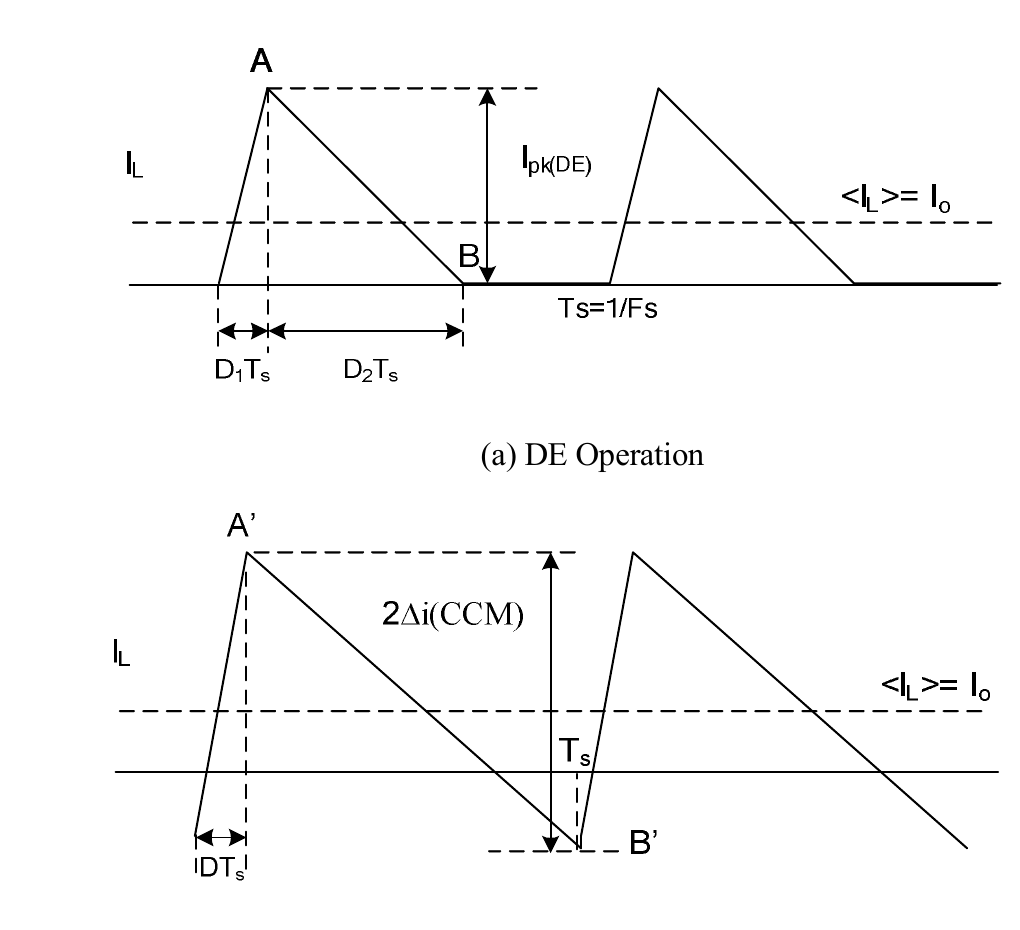
\includegraphics[width=0.68\textwidth]{literatur/gecici_de_ccm_akim_chen34.png}
  \caption{\diskaynaketiketi\ Diyot benzetimi (DE) ve sürekli iletim (CCM) kiplerinde endüktör akımının karşılaştırılması; Chen ve arkadaşlarından alınmıştır \citep{Chen2010}.}
  \label{fig:de-ccm-akim}
\end{figure}

Önceki tezde aynı kuramsal ayrım, sürekli ve süreksiz iletim için iki ayrı açıklayıcı şemayla verilmiştir. Tarihsel akışı ve eski yorumları korumak amacıyla söz konusu çalışma kopyaları Şekil~\ref{fig:onceki-tez-ccm-ters-akim} ve Şekil~\ref{fig:onceki-tez-dcm-akim} üzerinde birincil kaynaklı Şekil~\ref{fig:de-ccm-akim}'in hemen ardından sunulmuştur.

\begin{figure}[H]
  \centering
  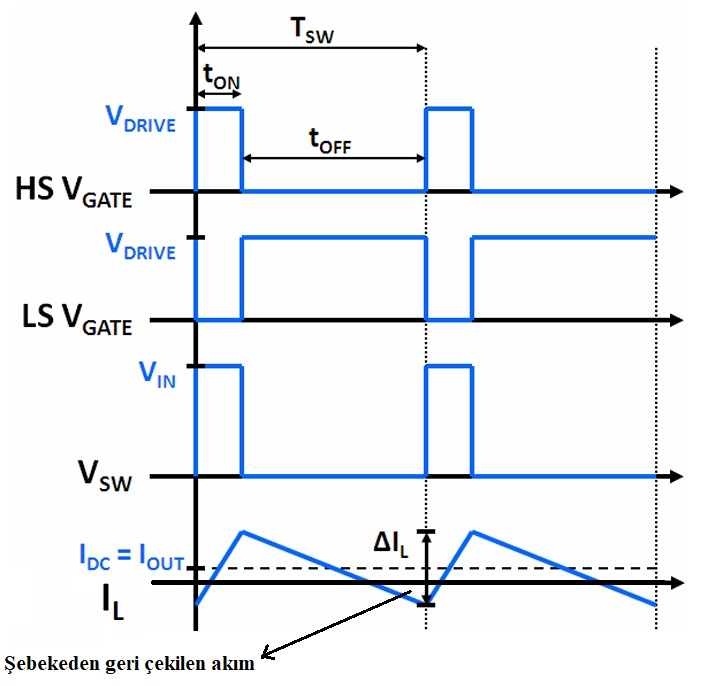
\includegraphics[width=0.72\textwidth]{sistem/onceki_tez_sekil3_11_ccm_ters_akim.jpeg}
  \caption{\eskitezetiketi\ Önceki tezin Şekil~3.11'inde verilen, senkron buck dönüştürücüde düşük görev oranındaki sürekli iletim ve ters akım şeması. Görsel nitel bir açıklama şemasıdır; ölçüm veya yeni benzetim sonucu değildir.}
  \label{fig:onceki-tez-ccm-ters-akim}
\end{figure}

Şekil~\ref{fig:onceki-tez-ccm-ters-akim}, yüksek ve alçak taraf kapı işaretleri tamamlayıcı biçimde sürülmeye devam ettiğinde endüktör akımının ortalama değerin altına indiği bölgeyi ve önceki tezde ``şebekeden geri çekilen akım'' olarak işaretlenen dolaşımı göstermektedir. Şemanın bölümdeki amacı, sürekli tamamlayıcı sürme ile negatif akım bölgesi arasındaki ilişkiyi görünür kılmaktır.

\begin{figure}[H]
  \centering
  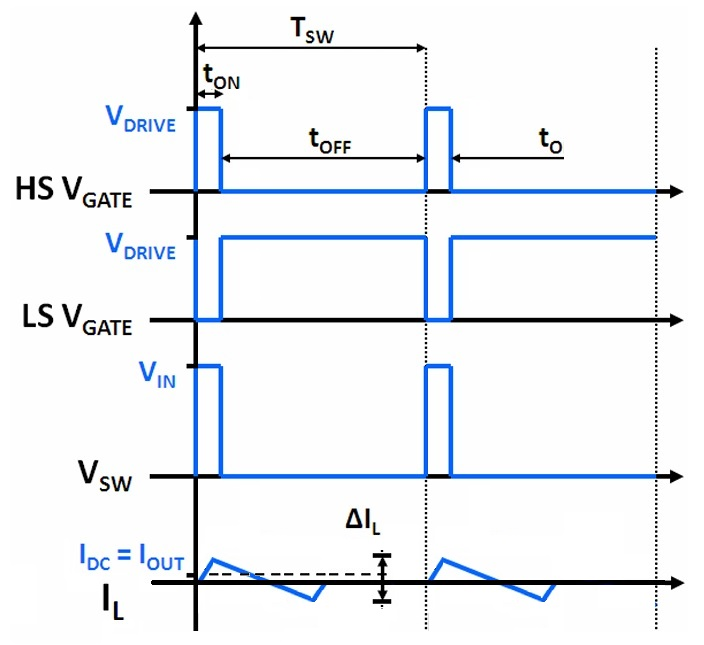
\includegraphics[width=0.72\textwidth]{sistem/onceki_tez_sekil3_12_dcm_akim.jpeg}
  \caption{\eskitezetiketi\ Önceki tezin Şekil~3.12'sinde verilen, senkron buck dönüştürücüde düşük görev oranındaki süreksiz iletim şeması. Görsel nitel bir açıklama şemasıdır; ölçüm veya yeni benzetim sonucu değildir.}
  \label{fig:onceki-tez-dcm-akim}
\end{figure}

Şekil~\ref{fig:onceki-tez-dcm-akim}, anahtarlama periyodunda $t_o$ ile gösterilen sürmesiz aralığın eklenmesini ve düşük yükte sürekli tamamlayıcı sürmenin kesilmesini açıklamak için kullanılmıştır. Her iki eski şemanın zaman ölçeği, devre parametreleri ve üretim yöntemi kayıtlı olmadığından görseller bağımsız performans kanıtı sayılmayacaktır. İleride gerçek MATLAB/Simulink modeliyle aynı kapı işaretleri ve endüktör akımı yeniden üretilerek Şekil~\ref{fig:de-ccm-akim} ile birlikte karşılaştırılacaktır.

\tezcalismanotu{D2-2 --- Eski Şekil 3.11--3.12'nin nihai kullanım kararı}{İki tarihsel CCM/DCM şeması eski tezin açıklama zincirini ezmemek amacıyla ana metinde tutulmuştur. Gerçek modelden kapı işaretleri, endüktör akımı ve sürmesiz aralık yeniden üretildiğinde eski görseller yeni sonuçlarla yan yana denetlenecek; yalnız aynı bilgiyi tekrarlıyorlarsa eke taşınacak, farklı bir mekanizma anlatıyorlarsa metin içi açıklaması genişletilecektir.}

Şebekeye bağlı T-tipi eviricide sıfır gerilim durumunu oluşturan nötr kol, akımın işaret değiştirmesine izin verdiğinde benzer bir senkron alçaltıcı davranışı gösterebilir. Nötr anahtarın susturulması ters akım yolunu keserken faz düğümünün doğal diyot yolları üzerinden farklı bir gerilim durumuna geçmesine neden olur. Sonuç olarak kayıp azalması ile anahtarlama darbe dizisinin değişmesi aynı fiziksel müdahalenin iki sonucudur. Literatürdeki genel süreksiz iletim bilgisi ters akımı açıklamak için gerekli kuramsal temeli sağlasa da T-tipi faz kolunda oluşan gerilim hatasının üçüncü harmonik etkisini ve şebeke akım kontrolüyle etkileşimini tek başına açıklamamaktadır.

\tezcalismanotu{D2-3 --- Eski FV, verim ve THD kayıtlarının veri denetimi}{Eski Şekil~2.1--2.10 ile Tablo~2.1--2.4 yeni tezde birleşik profil, yeniden hesaplanan sınıf tablosu ve seçilmiş karşılaştırma görselleriyle temsil edilmiştir. Konum, panel eğimi/yönelimi, PVGIS sorgusu, meteorolojik veri kümesi ve zaman ağırlıkları bulunursa temsilî 144 nokta gerçek saatlik profille değiştirilecektir. Ticari evirici kaydının cihaz modeli, analizör, ölçüm penceresi ve ham dosyası bulunamazsa ilgili sayı ve grafik yalnız tarihsel motivasyon olarak kalacak; Şekil~\ref{fig:fv-yil-saat-yuzeyi} ana metinde tutulacaksa en az 300 dpi veya vektör olarak yeniden üretilecektir.}

\section{Şebeke Akım Kontrolü ve İleri Besleme Yaklaşımları}

Şebekeye bağlı bir eviricide akım denetleyicisi, referans akım ile ölçülen akım arasındaki hatadan modülasyon gerilimi üretir. Senkron referans çerçevesi, durağan eksen PI kontrolü ve oransal-rezonans (PR) kontrolü yaygın seçenekler arasındadır. PR denetleyici, temel frekansta yüksek kazanç sağlayarak sinüzoidal referansın kalıcı durum hatasını azaltabilir; seçili harmoniklerde ek rezonans kolları da kullanılabilir \citep{Teodorescu2006PR,Teodorescu2011}. Faz kilitlemeli döngü veya eşdeğer bir eşzamanlama yapısı, şebeke faz ve frekans bilgisini üretir; tek fazlı sistemlerde ortogonal işaret üretimi ve dijital gecikmeler tasarımın parçasıdır \citep{Blaabjerg2006,Zhou2018}.

LCL filtre, daha küçük toplam endüktansla yüksek frekanslı anahtarlama bileşenlerini zayıflatabilmesine karşılık rezonans tepesi oluşturur. Pasif sönümleme direnç kaybı doğururken aktif sönümleme ölçülen akım veya gerilim işaretlerinden sanal empedans etkisi üretir. PR denetleyici ile LCL aktif sönümlemenin birlikte tasarımı, kapalı çevrim kutupları ve kararlılık marjları dikkate alınarak yapılmalıdır \citep{Zhang2014PR}. Şebeke gerilimi ileri beslemesi, ortak bağlantı noktasındaki bozucu gerilimin akıma taşınmasını azaltmak için modülasyon girişine ölçülen gerilimden türetilen bir terim ekler. Lu ve arkadaşları, dijital gecikmenin ileri besleme yolunu LCL rezonansı üzerinde aktif sönümleme veya negatif sönümleme üretebilen dinamik bir elemana dönüştürebildiğini göstermiştir \citep{Lu2016}. Zayıf şebeke koşullarını inceleyen Wang ve arkadaşları da şebeke empedansına bağlı pozitif geri besleme etkisinin faz marjını azaltabileceğini ve ileri besleme kanalının frekans seçici biçimde tasarlanması gerektiğini ortaya koymuştur \citep{Wang2024}.

Anahtar ölü zamanı, snubber ve parazitik kapasiteler de komut edilen gerilim ile gerçekleşen faz gerilimi arasında akım yönüne bağlı hata oluşturur. Zhang ve Xu, parazitik kapasitelerin anahtarlama kenarlarını sonlu eğimli hâle getirdiğini ve klasik darbe tabanlı ölü zaman kompanzasyonunun özellikle küçük akımlarda yetersiz kalabildiğini deneysel olarak göstermiştir \citep{Zhang2014Deadtime}. Dolayısıyla düşük güç harmonikleri yalnızca denetleyici bant genişliğinin değil; modülasyon, anahtar geçişi, akım yönü ve şebeke geriliminin ortak sonucudur.

Sin\textsuperscript{3} tabanlı yaklaşımın literatürdeki yerini doğru kurabilmek için üçüncü harmonik enjeksiyonu ile bozucu bastırma amaçlı ileri besleme ayrılmalıdır. Klasik üçüncü harmonik enjeksiyonu, faz referanslarına ortak mod bileşeni ekleyerek DA bara kullanım oranını artırmayı veya belirli anahtarlama harmoniklerini düzenlemeyi hedefler \citep{Holmes2003,Aghdam2013}. Tezde ele alınan Sin\textsuperscript{3} terimi ise nötr anahtar susturma yönteminin oluşturduğu üçüncü harmonik etkisine karşı, ölçülen şebeke işaretinden $\sin^3(\theta)=[3\sin(\theta)-\sin(3\theta)]/4$ özdeşliğiyle üretilen bir şekillendirme bileşenidir. Fourier gösterimi matematiksel temeli sağlarken terimin modülasyon girişine eklenmesi onu hata sinyalinden türetilen bağımsız bir geri besleme denetleyicisi yapmaz \citep{Oppenheim1997}.

İdeal doğrusal ve doyumsuz modelde dışsal ileri besleme terimi kapalı çevrimin karakteristik paydasını değiştirmeyebilir. Gerçek dönüştürücüde örnekleme, PWM gecikmesi, LCL rezonansı, sınırlayıcılar ve çalışma noktasına bağlı anahtarlama doğrusal olmayanlıkları söz konusu ideal ayrımı sınırlar. Periyodik çalışma noktaları çevresindeki frekans bağlaşımının incelenmesi gerektiğinde doğrusal zamanla periyodik modeller ve harmonik transfer fonksiyonları kullanılabilir \citep{Wereley1991,Liao2022}. Tez açısından temel gereksinim, Sin\textsuperscript{3} teriminin kontrolcü olarak adlandırılması değil; mevcut akım döngüsündeki konumunun, kapalı çevrim aktarımının ve düşük ile anma gücü koşullarındaki etkisinin açıkça doğrulanmasıdır.

\tezcalismanotu{D2-4 --- Literatür ve şekil kullanımının son denetimi}{Bölüm~4--7'nin sonuçları kesinleştiğinde literatür karşılaştırma tablosundaki ``tezde kalan sınır'' sütunu gerçek bulgularla yeniden eşleştirilecektir. Önceki tezden aktarılan ve dış kaynaktan uyarlanan her şekil için özgün kaynak, uyarlama derecesi, kullanım izni ve çözünürlük son teslimden önce kontrol edilecek; kaynak zinciri doğrulanamayan görseller bilimsel kanıt olarak bırakılmayacaktır.}

\section{Literatürün Karşılaştırmalı Değerlendirilmesi}

Tablo~\ref{tab:literatur-karsilastirma}, tezin üç katkı ekseniyle en yakından ilişkili çalışmaları kullanılan yapı, temel amaç, doğrulama düzeyi ve tez açısından kalan sınır üzerinden karşılaştırmaktadır. Karşılaştırma, bir çalışmanın genel başarısını değil, söz konusu tezin araştırma sorularını ne ölçüde kapsadığını göstermektedir.

\begin{longtable}{>{\raggedright\arraybackslash}p{0.18\textwidth} >{\raggedright\arraybackslash}p{0.20\textwidth} >{\raggedright\arraybackslash}p{0.24\textwidth} >{\raggedright\arraybackslash}p{0.26\textwidth}}
\caption{\diskaynaketiketi\ Tezle doğrudan ilişkili çalışmaların karşılaştırmalı sentezi.}\label{tab:literatur-karsilastirma}\\
\toprule
\textbf{Çalışma} & \textbf{Yapı ve odak} & \textbf{Doğrulama} & \textbf{Tez açısından kalan sınır} \\
\midrule
\endfirsthead
\caption[]{\diskaynaketiketi\ Tezle doğrudan ilişkili çalışmaların karşılaştırmalı sentezi (devamı).}\\
\toprule
\textbf{Çalışma} & \textbf{Yapı ve odak} & \textbf{Doğrulama} & \textbf{Tez açısından kalan sınır} \\
\midrule
\endhead
\bottomrule
\endfoot
Schweizer ve Kolar \citep{Schweizer2013} & Üç seviyeli T-tipi dönüştürücü; kayıp ve verim & Analitik kayıp hesabı ve donanım prototipi & Düşük güçte nötr kol ters akımı ve buna bağlı THD ele alınmamıştır. \\
Wang ve ark. \citep{Wang2020} & \SI{250}{\kilo\watt} SiC T-tipi evirici; güç yoğunluğu ve geçiş kayıpları & Kayıp modeli ve tam ölçekli prototip & Çalışma çekiş eviricisine ve yüksek güç tasarımına odaklanmıştır. \\
Chen ve ark. \citep{Chen2010} & Senkron buck; diyot benzetimi ve sürekli iletim & Analiz, benzetim ve deney & T-tipi şebeke eviricisinin sıfır durumu ve harmonik sonucu kapsanmamıştır. \\
Zhang ve Xu \citep{Zhang2014Deadtime} & Ölü zaman ve parazitik kapasite kompanzasyonu & Darbe modeli ve deney & Nötr anahtar susturma kaynaklı üçüncü harmonik hedeflenmemiştir. \\
Lu ve ark. \citep{Lu2016} & LCL eviricide şebeke gerilimi ileri beslemesi & Frekans alanı analizi ve deney & Sin\textsuperscript{3} tabanlı anlık şekillendirme ve düşük güç ters akımı ele alınmamıştır. \\
Wang ve ark. \citep{Wang2024} & Zayıf şebekede filtreli ileri besleme & Empedans modeli ve yarı fiziksel benzetim & Amaç şebeke empedansına uyumdur; anahtarlama kaynaklı üçüncü harmonik değildir. \\
Momayyezan ve ark. \citep{Momayyezan2016} & Yeniden yapılandırılabilir yüksek gerilim batarya dönüştürücüsü & Beş modüllü ölçekli prototip & Şebekeye bağlı üç seviyeli T-tipi evirici ve düşük güç yöntemiyle bütünleşmemiştir. \\
Farakhor ve ark. \citep{Farakhor2023} & Modüler yeniden yapılandırılabilir BESS ve hücre gücü yönetimi & Optimizasyon, benzetim ve laboratuvar prototipi & T-tipi/Vienna işlev paylaşımı ve şebeke akımı kalitesi hedeflenmemiştir. \\
Huang ve ark. \citep{Huang2024} & Anahtar tabanlı modüler yeniden yapılandırma ve dengeleme & Kayıp analizi ve ölçekli deney & İlaveli modül anahtarları kullanılmış; ortak T-tipi güç katı ele alınmamıştır. \\
\end{longtable}

\section{Araştırma Boşluğu}

Literatür taraması üç ayrı bilgi kümesinin gelişmiş olduğunu göstermektedir. İlk küme, T-tipi dönüştürücünün yüksek verim, güç yoğunluğu, anahtarlama geçişleri ve elektromanyetik uyumluluk özelliklerini açıklamaktadır \citep{Schweizer2013,Wang2020,Hizarci2021}. İkinci küme, hafif yükte ters akımı azaltan süreksiz iletim veya diyot benzetimi ilkelerini ve şebeke eviricilerindeki harmonik/ileri besleme problemlerini ele almaktadır \citep{Chen2010,Lu2016,Wang2024}. Üçüncü küme ise batarya modüllerini veya dönüştürücü elemanlarını farklı çalışma kiplerinde yeniden kullanan EDS mimarilerini geliştirmektedir \citep{Momayyezan2016,Farakhor2023,Huang2024}.

Kümeler arasındaki bağlantı sınırlıdır. T-tipi eviricinin düşük güçte sıfır durumunu oluşturan nötr kolun senkron buck benzeri ters akım mekanizması, aynı müdahalenin verim ve üçüncü harmonik üzerindeki karşıt etkileriyle birlikte yeterince incelenmemiştir. Ters akımı kesen anahtarlama değişikliği ile oluşan harmonik bileşeni, mevcut kapalı çevrimi bağımsız bir denetleyiciyle değiştirmeden şekillendiren Sin\textsuperscript{3} tabanlı ileri besleme terimi için de doğrudan bir karşılık belirlenememiştir. Yeniden yapılandırılabilir batarya literatürü işlev paylaşımının mümkün olduğunu gösterse de T-tipi evirici, Vienna PFC ve aktif batarya yönetimi işlevlerinin aynı yarı iletken yapı üzerinde birleştirilmesi; düşük güç anahtarlama ve şebeke akımı kalitesi ekseniyle ortak bir tez çerçevesinde ele alınmamıştır.

Belirlenen araştırma boşluğu, üç katkıyı tek bir sav altında birleştirmektedir: T-tipi dönüştürücünün anahtarlama durumları düşük güçte ters akımı azaltacak biçimde yeniden düzenlenebilir; ortaya çıkan harmonik ödünleşimi Sin\textsuperscript{3} tabanlı ileri besleme kompanzasyonuyla yönetilebilir; aynı topolojinin yarı iletkenleri EDS'nin farklı şarj--deşarj ve dengeleme kiplerinde yeniden görevlendirilebilir. Sonraki bölümlerde söz konusu sav; ortak sistem modeli, çalışma kipleri, elektriksel parametreler, kapalı çevrim analizleri ve erişilebilir benzetim/deney kanıtı üzerinden sınanacaktır.
